\documentclass[11pt,a4paper]{article}
\usepackage[margin=24mm]{geometry}
\usepackage[T1]{fontenc}
\usepackage[utf8]{inputenc}
\usepackage{lmodern}
\usepackage{amsmath,amssymb,amsthm}
\usepackage{booktabs}
\usepackage{longtable}
\usepackage{graphicx}
\usepackage{float}
\usepackage{xcolor}
\usepackage{enumitem}
\usepackage{microtype}
\usepackage{url}
\usepackage[colorlinks=true,linkcolor=linkblue,citecolor=linkblue,urlcolor=linkblue]{hyperref}
\definecolor{linkblue}{RGB}{20,60,140}
\graphicspath{{./}{figs/}{paper09_cod_certification_v44_src/figs/}}
\setlist{nosep}
\theoremstyle{plain}
\newtheorem{theorem}{Theorem}[section]
\newtheorem{proposition}[theorem]{Proposition}
\newtheorem{corollary}[theorem]{Corollary}
\newtheorem{lemma}[theorem]{Lemma}
\theoremstyle{definition}
\newtheorem{definition}[theorem]{Definition}
\theoremstyle{remark}
\newtheorem{remark}[theorem]{Remark}
\newcommand{\R}{\mathbb{R}}
\newcommand{\safe}{W_0}
\newcommand{\LRP}{\theta}
\newcommand{\Cstar}{C^{*}}
\newcommand{\Cvac}{C_{\mathrm{vac}}}
\newcommand{\gmax}{g_{\max}}
\newcommand{\Hstar}{H^{*}}
\newcommand{\Pbar}{\bar P}
\newcommand{\Tcert}{T_{\mathrm{cert}}}
\newcommand{\Tempty}{T_{\mathrm{empty}}}
\newcommand{\kt}{\,\mathrm{kt}}
\newcommand{\ft}{\,\mathrm{ft}}
\newcommand{\dd}{\mathrm{d}}
\newcommand{\nchecks}{77}
\title{\textbf{Certifying threshold management in one dimension:\\ closed-loop robust kernels for the Northern cod limit reference point and the Edwards Aquifer index well}}
\author{Ali Abaee}
\date{15 October 2026}
\begin{document}
\maketitle

\begin{abstract}
\noindent
Threshold rules promise that a resource remains above a limit, but simulation-based assessments usually estimate survival probabilities rather than establish a guarantee under a specified model class. We derive closed-loop robust viability kernels for one-dimensional monotone maps and apply the results, under protocols frozen on 2026-08-26, to Northern cod (NAFO 2J3KL; limit reference point $\theta=884.6$ kt) and Edwards Aquifer J-17 (triggers at 618 and 660 ft). For a continuous, strictly increasing map with a non-binding ceiling, the finite-horizon kernel has a computable lower boundary; over increasing horizons, the kernels are either the whole safe set, converge to a half-line above the smallest fixed point, or become empty at a finite horizon. For the Schaefer cod map, the regimes are governed by $C^*=g(\theta)-|e|$ and $C_{\mathrm{vac}}=g_{\max}-|e|$; for the affine aquifer map, by its worst-floor attractor. A staged rule affects protection at a threshold only through the control active at that threshold.

For cod, the q10 floor supports a constructive bound of $91.6$ kt, whereas the q05 and worst floors do not make the LRP self-viable. Exact bounded-defect horizons range from 8--13 years under the worst and q05 floors and 12--28 years under q10; the registered Lipschitz certificate gives 5--7 years. For the aquifer, a flat pumping cut of at least 7.2\% secures 618 ft; on observed heads the Stage-I rule supplies 3.3\% more than a flat 90\% cap at matched protection. No admissible rule secures 660 ft, even at zero pumping. At 618 ft, the declared-defect horizon is three years for positive-pumping rules and four at zero pumping; the out-of-sample defect reduces these to two and three years, respectively. The exact recursion extends cod horizons but leaves aquifer horizons unchanged, while recording boundary departures for staged controls and for zero pumping at the shortest horizons. Neither system admits an indefinite certificate under its declared defect. The framework links the catch-sensitive cod horizon to curvature away from the LRP and the aquifer horizon to the defect-to-contraction margin against its ceiling. An independent core reproduces 926 comparisons with the registered campaign artefacts; the data, protocols, code and verification record are distributed with the manuscript.
\end{abstract}

\noindent\textbf{Keywords:} viability kernel; robust invariance; limit reference point; critical period management; Northern cod; Edwards Aquifer; certification; model defect; reassessment cadence.

\section{Introduction}\label{sec:intro}

A threshold rule promises that a state variable will be held above a line. The 2016 Northern cod assessment fixed the limit reference point (LRP) at the 1983--1989 mean spawning stock biomass, $\LRP=884.6$ kt, and the Canadian precautionary framework attaches catch consequences to crossing it \cite{DFO2009,DFO2016}. The Edwards Aquifer Authority manages pumping through staged cuts triggered when the J-17 index well falls below 660, 650, 640 and 630 ft above mean sea level, with 618 ft the elevation below which spring flows and the endangered-species commitments of the Habitat Conservation Plan are in jeopardy \cite{EAA2024,EARIP2021,NRC2015}. In both cases the rule is stated as a guarantee, but the evidence offered for it is probabilistic: stochastic projections, management strategy evaluation, scenario ensembles \cite{Butterworth2007,Punt2016}. Those tools estimate how often the threshold holds. They do not answer the question the rule poses, which is whether the threshold can be held against everything a fitted model admits---whether it can be \emph{certified}.

Viability theory supplies the right object for that question. The viability kernel of a constraint set under a controlled dynamical system is the set of states from which the constraint can be maintained for ever \cite{Aubin1991}; its finite-horizon and robust variants are the states from which it can be maintained for $T$ steps, or against a class of disturbances \cite{BertsekasRhodes1971,RegnierDeLara2015}. The theory has been applied to fisheries and groundwater \cite{Bene2001,Martinet2007,Doyen2012,Krawczyk2013,Pereau2018,Pereau2019,Oubraham2018}, usually with numerically approximated kernels in two or more dimensions. The present paper takes a different route: it stays in one dimension, where the kernel of a threshold under a monotone map can be written down, and uses the closed form to say exactly what a frozen model does and does not establish about a rule.

Two systems are treated under one frame. They were chosen for contrast rather than similarity. The cod map is expansive at its reference point---the slope of the one-step map at the LRP is $F'(\LRP)=1.153$---so disturbances are amplified near the line the rule is meant to protect; the aquifer map is a contraction ($a=0.746$), so disturbances decay. The cod residuals are dominated by the 1991--1992 collapse years, which are seven to ten residual standard deviations from zero; the aquifer residuals are small in sample and larger out of sample. The cod safe set has no upper limit that matters; the aquifer has a ceiling at 710 ft that the backward recursion runs into. Everything that follows was computed under protocols frozen before the computations were made (both on 2026-08-26); the protocols are reproduced in the supplement.

The paper makes four contributions.

\begin{enumerate}[leftmargin=2em]
\item \emph{A closed-form certification frame for one-dimensional threshold management} (Section~\ref{sec:frame}). Theorem~\ref{thm:kernel} characterises the $T$-step and infinite-horizon closed-loop kernels of a threshold under any strictly increasing map with a non-binding ceiling: the kernel is the whole safe set, a half-line above the smallest fixed point, or empty beyond an explicit finite horizon. For a surplus-production stock the characterisation collapses to two constants, $\Cstar=g(\LRP)-|e|$ and $\Cvac=\gmax-|e|$ (Corollary~\ref{cor:cod}); for an affine aquifer map to one attractor and a closed-form emptying horizon (Corollary~\ref{cor:edw}). Proposition~\ref{prop:stage} shows that a staged rule acts on a threshold only through the stage active at that threshold.
\item \emph{An exact treatment of model defect} (Theorem~\ref{thm:exact}, Propositions~\ref{prop:lip}--\ref{prop:finite}). The registered protocols certified against a uniform model defect $\varepsilon$ by inflating the threshold with a Lipschitz accumulation $r_T$. We show that the exact robust kernel of the bounded-defect class is computable by the same interval recursion, that the Lipschitz certificate coincides with it for affine maps wherever the recursion binds, and that it is conservative for maps whose slope falls away from the threshold. For cod the exact kernel extends the horizon and makes it catch-sensitive; for the aquifer it leaves the horizon unchanged, although boundaries depart from the Lipschitz certificate at zero pumping for $T=1,2$ and under the staged rules. In both systems the certified horizon is finite for every admissible rule, and the condition for an indefinite certificate is stated and shown to fail.
\item \emph{Resolved answers for two managed systems} (Sections~\ref{sec:cod}--\ref{sec:edwards}, Table~\ref{tab:resolved}). For cod: the LRP is self-viable under constant catches up to $91.6$ kt under the 10th-percentile residual floor and under no catch at all under the 5th-percentile or worst floors; the Stage-I rule, the declared cascade and a flat 60-kt cap have identical kernels; the constructive bound is identified from the data even though the carrying capacity is not. For the aquifer: 618 ft is secured by any flat cut of at least $7.2\%$; the Stage-I rule is retained against the flat family because it ties the 90\% cap in protection and supplies $3.3\%$ more water; the 660-ft trigger cannot be held from itself under any recharge floor even with zero pumping; and the 2004 out-of-sample residual exceeds the declared defect, reducing the horizon for positive-pumping rules from three to two years while zero pumping retains three.
\item \emph{A cross-system reading of the certified horizon} (Section~\ref{sec:synthesis}). The horizons are finite but differ in their margins: under the cod Lipschitz certificate they are six years under the worst/q05 floors and seven under q10 for catches up to 150 kt, while the exact kernels extend to 8--13 and 12--28 years, respectively. For the aquifer the declared-defect horizon is three years for positive-pumping rules (four at zero pumping), and the out-of-sample horizon is two/three. The six-year International Whaling Commission Implementation Review cycle matches the registered cod certificate for catches up to 180 kt under the worst/q05 floors; the aquifer result under the out-of-sample defect calls for a shorter two-year reassessment interval.
\end{enumerate}

The paper is organised as follows. Section~\ref{sec:frame} develops the frame. Sections~\ref{sec:cod} and \ref{sec:edwards} apply it to cod and to the aquifer, each with its stochastic and identification layers. Section~\ref{sec:synthesis} reads the two systems together. Section~\ref{sec:discussion} states limitations, Section~\ref{sec:verification} the verification record, Section~\ref{sec:related} the relation to prior work, and Section~\ref{sec:conclusion} concludes. The supplement (S1--S14) carries the data, the full kernel tables, the stochastic and bootstrap grids, the Edwards replays and the symbol list.

\section{A certification frame for one-dimensional threshold management}\label{sec:frame}

\subsection{Objects}\label{sec:objects}

The state is a scalar $x\in X=[x_{\mathrm{lo}},x_{\mathrm{hi}}]$ (spawning biomass in kt; index-well head in ft). A \emph{threshold} $\LRP\in X$ defines the safe set $\safe=[\LRP,x_{\mathrm{hi}}]$; the ceiling $x_{\mathrm{hi}}$ is the top of the model's declared domain, and the state is clamped there rather than failed. A \emph{rule} (policy) is a map $\pi:X\to U$ from state to control, piecewise constant with finitely many jump points in all cases treated here. The one-step dynamics are
\begin{equation}\label{eq:dyn}
x_{t+1}=\Phi(x_t,\pi(x_t),w_t),
\end{equation}
where $w_t$ is a scalar disturbance---the residual of the fitted map for cod, the annual recharge for the aquifer---and $\Phi$ is non-decreasing in $w$. An \emph{uncertainty class} is a set of admissible disturbance sequences; the classes used here are \emph{floor classes} $\{w_t\ge \underline w\ \forall t\}$ with $\underline w$ the minimum, 5th or 10th percentile of the fit-window disturbances (``worst'', ``q05'', ``q10''). The \emph{floor map} is $F_\pi(x)=\Phi(x,\pi(x),\underline w)$.

\begin{definition}[closed-loop kernels]\label{def:kernel}
For a rule $\pi$ and a class $\mathcal W$, the $T$-step closed-loop robust kernel is
$W_T(\pi,\mathcal W)=\{x\in\safe:\ x_t\in\safe\ \text{for } t=0,\dots,T \text{ for every } (w_t)\in\mathcal W\}$, and $W_\infty=\bigcap_T W_T$. Its lower boundary is $b_T=\inf W_T$ ($b_T=\infty$ if $W_T=\emptyset$).
\end{definition}

\begin{lemma}[floor reduction]\label{lem:floor}
If $\Phi$ is non-decreasing in $w$ and $\mathcal W$ is a floor class, then $W_T(\pi,\mathcal W)$ equals the deterministic $T$-step viability kernel of $\safe$ under the floor map $F_\pi$, i.e.\ the sets generated by
\begin{equation}\label{eq:rec}
W_0=\safe,\qquad W_{t+1}=\{x\in\safe:\ F_\pi(x)\in W_t\}.
\end{equation}
\end{lemma}
\begin{proof}
Fix $x$ and a disturbance sequence in the class. By monotonicity in $w$ and induction, the realised state dominates the floor orbit, $x_t\ge F_\pi^{\,t}(x)$, provided the floor orbit stays in the region on which $F_\pi$ is monotone in $x$ (verified below for each map). Hence the floor sequence is the worst admissible one, and $x$ is $T$-step safe for every admissible sequence iff it is $T$-step safe under the floor map, which is \eqref{eq:rec}.
\end{proof}

The recursion \eqref{eq:rec} is exact and cheap in one dimension. If $F_\pi$ is strictly increasing on each piece of $\pi$, the preimage of an interval under a piece is an interval obtained from the branch inverse, so every $W_t$ is a finite union of closed intervals and \eqref{eq:rec} is a finite computation (the registered runners and the independent core of Section~\ref{sec:verification} both implement it this way).

\subsection{The kernel of a monotone map above a threshold}

\begin{theorem}[kernel structure]\label{thm:kernel}
Let $F:\safe\to\R$ be continuous and strictly increasing with $F(x_{\mathrm{hi}})\le x_{\mathrm{hi}}$, and let $W_t$ be generated by \eqref{eq:rec}. Then:
\begin{enumerate}[label=(\alph*)]
\item each $W_t$ is a closed interval $[b_t,x_{\mathrm{hi}}]$ or empty, with $b_0=\LRP$ and $b_{t+1}=\max\{\LRP,F^{-1}(b_t)\}$, where $F^{-1}(y)=\inf\{x\in\safe:F(x)\ge y\}$ and $F^{-1}(y)=\infty$ if $F(x_{\mathrm{hi}})<y$; the sequence $b_t$ is non-decreasing;
\item if $F(\LRP)\ge\LRP$ then $W_t=\safe$ for all $t$ (\emph{whole safe set});
\item if $F(\LRP)<\LRP$ and $F$ has a fixed point in $(\LRP,x_{\mathrm{hi}}]$, let $x_f$ be the smallest; then $b_t\uparrow x_f$ with $b_t<x_f$ for every finite $t$, and $W_\infty=[x_f,x_{\mathrm{hi}}]$ (\emph{half-line});
\item if $F(\LRP)<\LRP$ and $F$ has no fixed point in $(\LRP,x_{\mathrm{hi}}]$, then $W_T=\emptyset$ for all $T\ge\Tempty=\min\{T:F^{T}(x_{\mathrm{hi}})<\LRP\}<\infty$ (\emph{empty beyond a finite horizon}).
\end{enumerate}
\end{theorem}
\begin{proof}
(a) By induction. If $W_t=[b_t,x_{\mathrm{hi}}]$ then $F(x)\in W_t$ iff $b_t\le F(x)\le x_{\mathrm{hi}}$; the upper inequality holds on $\safe$ because $F(x)\le F(x_{\mathrm{hi}})\le x_{\mathrm{hi}}$, and by strict monotonicity the lower one holds iff $x\ge F^{-1}(b_t)$. Monotonicity of $b_t$: $b_1\ge\LRP=b_0$, and $b_t\ge b_{t-1}$ implies $F^{-1}(b_t)\ge F^{-1}(b_{t-1})$. (b) $F(\LRP)\ge\LRP$ gives $F^{-1}(\LRP)\le\LRP$, so $b_1=\LRP$ and inductively $b_t=\LRP$. (c) On $[\LRP,x_f)$ we have $F(x)<x$ (continuity, $F(\LRP)<\LRP$, no fixed point), so an orbit started there decreases strictly and, having no fixed point to converge to in $[\LRP,x_f)$, leaves $\safe$ in finite time; hence $b_\infty\ge x_f$. Conversely $[x_f,x_{\mathrm{hi}}]$ is forward invariant ($F(x_f)=x_f$, $F$ increasing, $F(x_{\mathrm{hi}})\le x_{\mathrm{hi}}$), so $b_t\le x_f$ for all $t$. Strictness: $b_t<x_f$ implies $b_{t+1}=\max\{\LRP,F^{-1}(b_t)\}<F^{-1}(x_f)=x_f$. (d) Since $F$ is increasing, $F^{t}(x)\le F^{t}(x_{\mathrm{hi}})$ for all $x\in\safe$, so $W_T\neq\emptyset$ iff $x_{\mathrm{hi}}\in W_T$ iff $F^{t}(x_{\mathrm{hi}})\ge\LRP$ for $t\le T$. The orbit of $x_{\mathrm{hi}}$ is non-increasing and cannot converge inside $\safe$ (no fixed point there), so it crosses $\LRP$ at a finite $\Tempty$.
\end{proof}

The theorem says that a monotone one-dimensional threshold problem has exactly three outcomes, and that the outcome is decided by two scalar facts: the sign of $F(\LRP)-\LRP$ and the existence of a fixed point above $\LRP$. The two corollaries record what those facts are for the two model families used here.

\begin{corollary}[surplus-production stock]\label{cor:cod}
Let $F_C(S)=S+g(S)-C-|e|$ with $g$ continuous, $g$ increasing on $[0,S_{\mathrm{pk}}]$ and decreasing beyond, $\gmax=g(S_{\mathrm{pk}})$, $\LRP<S_{\mathrm{pk}}$, $F_C$ strictly increasing on $\safe$ and $g(x_{\mathrm{hi}})\le C+|e|$. Define
\[
\Cstar=g(\LRP)-|e|,\qquad \Cvac=\gmax-|e|.
\]
Then for a constant catch $C\ge0$: $W_\infty=\safe$ iff $C\le\Cstar$; $\safe\supsetneq W_\infty=[s_-(C+|e|),x_{\mathrm{hi}}]\neq\emptyset$ iff $\Cstar<C\le\Cvac$, where $s_-(\ell)$ is the smaller root of $g(S)=\ell$; and $W_T=\emptyset$ beyond a finite horizon iff $C>\Cvac$. The $T$-step boundaries follow from (a) with the branch inverse of $F_C$. For the Schaefer form $g(S)=rS(1-S/K)$: $\gmax=rK/4$, $s_\pm(\ell)=\tfrac K2\bigl(1\pm\sqrt{1-4\ell/(rK)}\bigr)$, $F_C'(S)=1+r(1-2S/K)$, and $F_C'(\LRP)>1$ iff $K>2\LRP$. For a proportional rule $C=\phi\,g(S)$ on $\safe$ the same statements hold with $g$ replaced by $(1-\phi)g$: whole safe set iff $\phi\le 1-|e|/g(\LRP)$, non-empty iff $\phi\le1-|e|/\gmax$.
\end{corollary}

\begin{corollary}[affine aquifer map]\label{cor:edw}
Let $F(H)=aH+b$ with $0<a<1$, $b=\alpha+\beta\underline R+\gamma P$, and attractor $\Hstar=b/(1-a)\le x_{\mathrm{hi}}$. Then $W_\infty=\safe$ iff $\Hstar\ge\LRP$; otherwise there is no fixed point above $\LRP$,
\[
b_T=\Hstar+\frac{\LRP-\Hstar}{a^{T}},\qquad \Tempty=\Bigl\lfloor\frac{\ln\bigl((x_{\mathrm{hi}}-\Hstar)/(\LRP-\Hstar)\bigr)}{\ln(1/a)}\Bigr\rfloor+1 .
\]
The half-line regime does not occur for a contraction: the kernel of a threshold above the attractor is the whole safe set or empty in finite time.
\end{corollary}
\begin{proof}
Both corollaries instantiate Theorem~\ref{thm:kernel}: $F_C(\LRP)\ge\LRP$ iff $g(\LRP)\ge C+|e|$; fixed points of $F_C$ solve $g(S)=C+|e|$, which has a root above $\LRP$ iff $C+|e|\le\gmax$ (then $s_-(C+|e|)>\LRP$ because $g(\LRP)<C+|e|$ and $g$ increases up to $S_{\mathrm{pk}}$). For the affine map the unique fixed point is $\Hstar$; $F(\LRP)\ge\LRP$ iff $\Hstar\ge\LRP$; $b_T$ follows from $F^{-1}(y)=(y-b)/a$ by induction, and $\Tempty$ is the first $T$ with $b_T>x_{\mathrm{hi}}$.
\end{proof}

\begin{proposition}[stage-at-threshold principle]\label{prop:stage}
Let $\pi$ be piecewise constant with jump points $s_1<s_2<\dots$ and let $F_\pi$ be strictly increasing on each piece. (i) The kernels $W_T(\pi)$ of a threshold $\LRP$ depend on $\pi$ only through its values on $\safe=[\LRP,x_{\mathrm{hi}}]$; two rules that agree on $\safe$ have identical kernels of $\LRP$ at every horizon. (ii) $W_\infty(\pi)=\safe$ iff $F_\pi(\LRP)\ge\LRP$ and $F_\pi(s_j^{+})\ge\LRP$ at every jump point $s_j\in\safe$, i.e.\ iff the stage active at the threshold holds it and no higher stage dips below it. (iii) In particular, if $\pi$ coincides on $\safe$ with a constant control $u_\LRP$, then $W_T(\pi)=W_T(u_\LRP)$ for all $T$, and the stages prescribed below $\LRP$ are irrelevant to the certification of $\LRP$.
\end{proposition}
\begin{proof}
(i) is immediate from \eqref{eq:rec}, which only evaluates $F_\pi$ on $\safe$. (ii) $\safe$ is forward invariant iff $\inf_{x\in\safe}F_\pi(x)\ge\LRP$; on each piece the infimum is attained at the left end by monotonicity. (iii) is (i).
\end{proof}

The proposition is elementary, but it is the statement that most often contradicts the design intent of staged rules. A cascade that cuts harder as the state falls further below a trigger protects the \emph{lower} lines it draws; it does nothing for the trigger itself that the first stage does not already do. In Section~\ref{sec:cod} this makes the Stage-I rule, the declared cascade and a flat 60-kt cap indistinguishable at the LRP; in Section~\ref{sec:edwards} it makes the Stage-I rule tie the flat 80\% cap at 618 ft and Critical Period Management tie the flat 60\% cap.

\subsection{Model defect: exact robust kernel and the Lipschitz certificate}\label{sec:defect}

Floor classes bound the disturbance; they do not bound the error of the fitted map itself. The registered protocols declared a uniform defect $\varepsilon$ equal to the largest absolute fit-window residual and certified against the class $\mathcal D_\varepsilon$ of all maps $F+\delta_t$ with $\sup_x|\delta_t(x)|\le\varepsilon$, time-varying and state-dependent, applied on top of the floor class.

\begin{theorem}[exact bounded-defect kernel]\label{thm:exact}
For a floor map $F$ (clamped at $x_{\mathrm{hi}}$) and the defect class $\mathcal D_\varepsilon$, the $T$-step robust kernel of $\safe$ is generated by
\begin{equation}\label{eq:exact}
W^{\varepsilon}_0=\safe,\qquad W^{\varepsilon}_{t+1}=\bigl\{x\in\safe:\ [\,F(x)-\varepsilon,\ \min\{F(x)+\varepsilon,x_{\mathrm{hi}}\}\,]\subset W^{\varepsilon}_t\bigr\}.
\end{equation}
If $F$ is strictly increasing on each piece, every $W^{\varepsilon}_t$ is a finite union of intervals computable from the branch inverses; for a single increasing branch with the ceiling non-binding, $W^{\varepsilon}_T=[b^{\varepsilon}_T,x_{\mathrm{hi}}]$ with $b^{\varepsilon}_0=\LRP$ and $b^{\varepsilon}_{t+1}=\max\{\LRP,F^{-1}(b^{\varepsilon}_t+\varepsilon)\}$.
\end{theorem}
\begin{proof}
A state is $(t{+}1)$-step robustly safe iff it is safe now and every successor the class allows is $t$-step robustly safe; the set of allowed successors of $x$ is the (clamped) interval $[F(x)-\varepsilon,F(x)+\varepsilon]$ because the defect is an arbitrary bounded perturbation at every step \cite{BertsekasRhodes1971,Aubin1991}. Nothing is lost in \eqref{eq:exact}: it is the dynamic-programming characterisation of the kernel, not a bound on it. The interval form follows as in Theorem~\ref{thm:kernel}(a).
\end{proof}

\begin{proposition}[Lipschitz certificate]\label{prop:lip}
Let $a\ge\sup_{\safe}F'$ and $r_T=\varepsilon\sum_{k=0}^{T-1}a^{k}$, i.e.\ $r_T=\varepsilon(a^{T}-1)/(a-1)$ for $a\neq1$. Write $W_T(\LRP')$ for the nominal $T$-step kernel of a threshold $\LRP'$ under \eqref{eq:rec}.
\begin{enumerate}[label=(\roman*)]
\item (inner approximation) $W_T(\LRP+r_T)\subset W^{\varepsilon}_T$ for every $T$.
\item (affine case) If $F(x)=ax+b$ then $b^{\varepsilon}_T=\max\{\LRP,F^{-T}(\LRP+r_T)\}$: the exact boundary is the Lipschitz boundary without the inflation of the initial state. The two certificates coincide whenever the backward recursion binds.
\item (expansive concave case) If $F'$ is strictly decreasing on $\safe$ (as for the Schaefer map) and $W^{\varepsilon}_T\neq\emptyset$ with $T\ge2$, the inclusion in (i) is strict.
\end{enumerate}
\end{proposition}
\begin{proof}
(i) Let $x\in W_T(\LRP+r_T)$ and let $x_t$ be a realised orbit under some $F+\delta_t$. With $d_t=|x_t-F^{t}(x)|$ one has $d_{t+1}\le a\,d_t+\varepsilon$, so $d_t\le r_t\le r_T$ and $x_t\ge F^{t}(x)-r_T\ge\LRP$ for $t\le T$. (ii) For an affine map $F^{-t}(y+a^{t}\varepsilon)=F^{-t}(y)+\varepsilon$, so by induction $F^{-1}\bigl(F^{-t}(\LRP+r_t)+\varepsilon\bigr)=F^{-(t+1)}(\LRP+r_t+a^{t}\varepsilon)=F^{-(t+1)}(\LRP+r_{t+1})$, which is the recursion of Theorem~\ref{thm:exact}. (iii) The exact recursion propagates the defect through $F^{-1}$ evaluated at $b^{\varepsilon}_t+\varepsilon>\LRP$, where the local slope is strictly below $a=F'(\LRP)$; the Lipschitz recursion charges the slope $a$ at every step, so for $T\ge2$ its boundary is strictly higher wherever both are finite.
\end{proof}

\begin{proposition}[finite certified horizons]\label{prop:finite}
Let $\Tcert=\max\{T:W^{\varepsilon}_T\neq\emptyset\}$ for a constant control.
\begin{enumerate}[label=(\roman*)]
\item (surplus-production stock) $\Tcert<\infty$ iff $C+|e|+\varepsilon>\gmax$, i.e.\ iff $C>\Cvac-\varepsilon$. If $\varepsilon\ge\Cvac$ no catch level, including zero, is certifiable indefinitely. Under the Lipschitz certificate, in addition, $\Tcert\le\bigl\lfloor\ln\bigl(1+(x_{\mathrm{hi}}-\LRP)(a-1)/\varepsilon\bigr)/\ln a\bigr\rfloor$ for every rule.
\item (affine contraction) $\Tcert<\infty$ iff $\Hstar<\LRP+\varepsilon/(1-a)$; a rule is certifiable indefinitely iff its worst-floor attractor clears the threshold by at least $r_\infty=\varepsilon/(1-a)$.
\end{enumerate}
\end{proposition}
\begin{proof}
(i) By Theorem~\ref{thm:exact} the exact boundary obeys $b_{t+1}=F^{-1}(b_t+\varepsilon)$, which has a fixed point iff $F(x)-\varepsilon=x$ has a solution above $\LRP$, i.e.\ $g(x)=C+|e|+\varepsilon$, possible iff the right side is at most $\gmax$. Without a fixed point $b_t$ increases without bound and passes $x_{\mathrm{hi}}$ at a finite $T$. The Lipschitz bound follows from $W_T(\LRP+r_T)=\emptyset$ once $\LRP+r_T>x_{\mathrm{hi}}$. (ii) For the affine map, $b^{\varepsilon}_T=\Hstar+(\LRP+r_T-\Hstar)/a^{T}$ when the recursion binds; since $r_T\uparrow r_\infty$ and $a^{-T}\to\infty$, $b^{\varepsilon}_T$ exceeds $x_{\mathrm{hi}}$ for large $T$ iff $\LRP+r_\infty-\Hstar>0$; if $\Hstar\ge\LRP+r_\infty$ the recursion never binds and $W^{\varepsilon}_T\supset[\LRP+r_T,x_{\mathrm{hi}}]$ for all $T$.
\end{proof}

\subsection{Securability, retention and the frozen protocol}

\begin{theorem}[securability margin]\label{thm:margin}
Suppose the control enters the floor map monotonically and let $F_0$ be the floor map under the most protective admissible control (zero catch; zero pumping). A threshold $\LRP$ admits a rule with $W_\infty=\safe$ iff $F_0(\LRP)\ge\LRP$. For the surplus-production stock this reads $g(\LRP)\ge|e|$ ($\Cstar\ge0$); for the affine aquifer map it reads $\Hstar_0=(\alpha+\beta\underline R)/(1-a)\ge\LRP$, and the minimal flat cut securing $\LRP$ is $1-\rho^{*}$ with
$\rho^{*}=\bigl(\LRP(1-a)-\alpha-\beta\underline R\bigr)/(\gamma\Pbar)$.
\end{theorem}
\begin{proof}
If $F_0(\LRP)<\LRP$ then $F_\pi(\LRP)\le F_0(\LRP)<\LRP$ for every admissible rule, and Theorem~\ref{thm:kernel}(c,d) excludes the whole safe set. If $F_0(\LRP)\ge\LRP$ the most protective rule attains it by Theorem~\ref{thm:kernel}(b). The cut formula solves $\Hstar(\rho\Pbar)=\LRP$.
\end{proof}

A \emph{reading} is a pair (floor class, threshold). Following the registered protocols, a staged rule is \emph{retained} against the flat family at a reading if (a) it is at least as protective as business-as-usual at every horizon there, and (b) it supplies at least as much control (catch; pumping) as every flat cap that is at least as protective as itself. Clause (a) is a dominance condition on kernels, clause (b) a supply comparison on the observed state history; both are decided, not estimated.

The protocols fix, before any kernel is computed: the data extracts and their provenance; the fit window and the out-of-sample audit window; the model form and the estimator; the residual convention; the floor classes and the quantile convention (linear interpolation); the defect $\varepsilon$ as the largest absolute fit-window residual with the out-of-sample maximum reported as an audit; the thresholds; the ceiling; the policy family; the horizon grid; and the retention rule. Everything downstream is a theorem about those declarations.

\section{Northern cod: the limit reference point under a Schaefer map}\label{sec:cod}

\subsection{Data, map and declarations}\label{sec:cod-data}

The state is spawning stock biomass $S_t$ (kt) from the 2016 assessment (NCAM, Table A2; 1983--2015), the control is the annual catch $C_t$ (kt) from the reconstructed landings of Schijns et al.~\cite{Schijns2021}, and the LRP is $\LRP=884.6$ kt, the 1983--1989 mean \cite{DFO2016}. The map is the Schaefer surplus-production step with source-year catch,
\begin{equation}\label{eq:cod-map}
S_{t+1}=S_t+rS_t\Bigl(1-\frac{S_t}{K}\Bigr)-C_t+e_{t+1},
\end{equation}
fitted by one-step least squares on the 24 transitions 1983$\to$1984 to 2006$\to$2007 with $K$ constrained to the box $[\max S+10,\,5000]$ kt. The minimiser is $r=0.2369$ with $K$ at the upper edge of the box; the profile of the sum of squares in $K$ is flat to within 2.7\% from 1500 kt to the top of a 50\,000-kt grid (Section~\ref{sec:cod-ident}), so $K$ is unidentified from above and every statement below is conditional on the declared box. The fit residuals have standard deviation 114.9 kt and lag-one autocorrelation 0.554; their minimum, 5th and 10th percentiles are $-329.0$, $-287.4$ and $-80.9$ kt, which define the three floor classes. The two collapse transitions, 1991$\to$1992 and 1992$\to$1993 ($-329.0$ and $-323.5$ kt), are the only residuals below $-172.5$ kt; the 10th-percentile floor sits between the second and third order statistics, which is why that class, and only that class, is sensitive to the quantile convention (SI Section~S2). The eight out-of-sample transitions 2008--2015 have standard deviation 28.1 kt and largest absolute residual 46.7 kt (2014), inside the declared defect $\varepsilon=329.0$ kt. Figure~\ref{fig:data}a shows the series and the residuals. Table~\ref{tab:inputs} lists every declared quantity for both systems.

\begin{table}[t]
\centering
\caption{Certification inputs for the two systems. Every quantity is fixed by the two intervention protocols frozen on 2026-08-26 and re-derived from the data files by the exact core (Section~\ref{sec:verification}). Floor classes are the minimum, 5th and 10th percentiles (linear interpolation) of the fitted residuals (cod) or of the fit-window recharge (Edwards).}
\label{tab:inputs}
\small
\resizebox{\textwidth}{!}{%
\begin{tabular}{lll}
\toprule
Quantity & Northern cod (2J3KL) & Edwards Aquifer (J-17) \\
\midrule
state $x$ & SSB $S$ (kt), NCAM 2016 & J-17 annual mean head $H$ (ft AMSL) \\
control $u$ & annual catch $C$ (kt) & annual pumping $P$ ($10^3$ ac-ft) \\
exogenous driver & none (residual only) & recharge $R$ ($10^3$ ac-ft), floor-classed \\
one-step map & $S' = S + rS(1-S/K) - C + e$ & $H' = aH + \alpha + \beta R + \gamma P + e$ \\
threshold(s) & LRP $\theta = 884.6$ kt & 618 ft (physical), 660 ft (institutional) \\
ceiling $x_{\mathrm{hi}}$ & 10\,000 kt & 710 ft \\
fit window / transitions & 1983--2007 / 24 & 1934--1990 / 56 \\
out-of-sample audit & 2008--2015 / 8 & 1991--2023 / 33 \\
parameters & $r=0.2369$, $K=5000$ (box edge) & $a=0.7461$, $\alpha=163.49$, $\beta=0.0198$, $\gamma=-0.02844$ \\
slope at threshold & $F'(\theta)=1.1531$ (expansive) & $a=0.7461$ (contracting) \\
residual SD (fit / OOS) & 114.9 / 28.1 kt & 5.60 / 8.40 ft \\
declared defect $\varepsilon$ (fit max) & 329.0 kt (1992) & 15.41 ft (1971) \\
OOS max $|$residual$|$ & 46.7 kt (2014); within $\varepsilon$ & 21.81 ft (2004); exceeds $\varepsilon$ \\
floor classes (worst / q05 / q10) & $|e| = 329.0$ / 287.4 / 80.9 kt & $R \ge 43.7$ / 166.5 / 179.1 \\
reference control level & $\bar C = 240$ kt (pre-1992 directed fishery) & $\bar P = 282.16$ (1934--1990 mean) \\
\bottomrule
\end{tabular}
}
\end{table}


The rule family is the one declared in the protocol: the moratorium-level removals $C=5$ kt (BAU); flat caps at $0$, $60$, $120$, $180$ and $240$ kt ($0$--$100\%$ of the pre-1992 directed fishery); the precautionary-framework Stage-I rule (60 kt at or above the LRP, zero below); the declared cascade (60/30/5/0 kt at the LRP, $0.75\,\LRP$ and $0.5\,\LRP$); two graded rules that \emph{raise} catch above the LRP (60 kt on $[\LRP,1.25\LRP)$ and 90 kt above; 30/60/90 kt on three bands); and the proportional family $C=\phi\,g(S)$ with $\phi\in\{0.25,0.5,0.6,0.75\}$. The ceiling is $x_{\mathrm{hi}}=10\,000$ kt, far above any state and above the point $K(1+r)/2r=13\,054$ kt beyond which the map would cease to be increasing, so Theorem~\ref{thm:kernel} applies on the whole safe set.


\begin{figure}[t]\centering
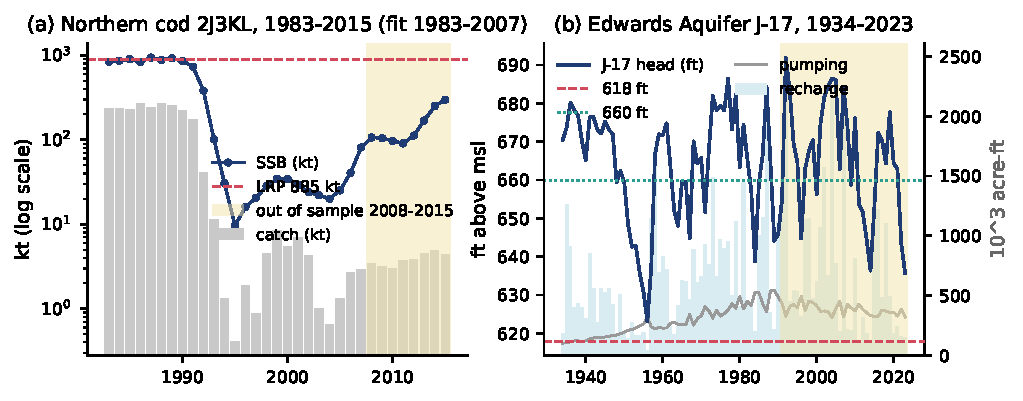
\includegraphics[width=\textwidth]{fig_data.pdf}
\caption{The two locked panels. (a)~Northern cod 2J3KL spawning stock biomass (NCAM, 2016 assessment) and reconstructed catch, 1983--2015, with the limit reference point $\LRP=884.6\kt$; the map is fitted on 1983--2007 and audited on the shaded 2008--2015 transitions. (b)~Edwards Aquifer J-17 annual mean elevation with the 618-ft and 660-ft triggers, total recharge and total pumping, 1934--2023; the map is fitted on 1934--1990 and audited on the shaded 1991--2023 transitions.}
\label{fig:data}
\end{figure}

\subsection{The three constants and the nominal kernels}\label{sec:cod-kernels}

Corollary~\ref{cor:cod} reduces every constant-catch question to two numbers. At the registered fit,
\[
g(\LRP)=172.46\kt,\qquad \gmax=\tfrac{rK}{4}=296.09\kt,\qquad F'(\LRP)=1+r\Bigl(1-\frac{2\LRP}{K}\Bigr)=1.1531,
\]
so under the 10th-percentile floor $\Cstar=172.46-80.87=91.59$ kt and $\Cvac=296.09-80.87=215.22$ kt. Under the 5th-percentile floor $\Cstar=-114.9$ kt and $\Cvac=8.7$ kt; under the perpetual-worst floor both are negative ($-156.5$ and $-32.9$ kt). Three facts about the reference point follow before any kernel is computed. First, the LRP is \emph{self-viable}---holds itself from itself---only under the q10 floor, and there under any constant catch up to $91.6$ kt. Second, under the q05 floor the only constant catches with a non-empty infinite-horizon kernel are those below $8.7$ kt, and the kernel they have is a half-line starting far above the LRP ($b_\infty=2219.6$ kt for BAU); under the worst floor every kernel is empty in finite time, because the single 1992 residual exceeds the maximum surplus the fitted map can produce. Third, the largest-residual floor is \emph{vacuous} in the precise sense of Theorem~\ref{thm:kernel}(d): it does not rank rules, it excludes all of them.

\begin{table}[t]
\centering
\caption{Northern cod: nominal kernel boundaries at horizons $T=1$, $5$ and $\infty$.}
\label{tab:cod-kernels}
\small
\resizebox{\textwidth}{!}{%
\begin{tabular}{lrrrrrrrrr}
\toprule
Policy & \multicolumn{3}{c}{worst ($|e|=329.0$)} & \multicolumn{3}{c}{q05 ($|e|=287.4$)} & \multicolumn{3}{c}{q10 ($|e|=80.9$)} \\ & $b_1$ & $b_5$ & $b_\infty$ & $b_1$ & $b_5$ & $b_\infty$ & $b_1$ & $b_5$ & $b_\infty$ \\
\midrule
zero catch & 1021.1 & 1431.6 & $\emptyset$ & 984.6 & 1280.8 & 2070.9 & 884.6 & 884.6 & 884.6 \\
BAU (5 kt) & 1025.5 & 1450.0 & $\emptyset$ & 989.0 & 1298.7 & 2219.6 & 884.6 & 884.6 & 884.6 \\
flat 60 kt & 1073.8 & 1656.7 & $\emptyset$ & 1037.2 & 1499.6 & $\emptyset$ & 884.6 & 884.6 & 884.6 \\
flat 120 kt & 1126.8 & 1891.7 & $\emptyset$ & 1090.0 & 1727.6 & $\emptyset$ & 909.2 & 979.9 & 1082.3 \\
flat 180 kt & 1180.0 & 2137.6 & $\emptyset$ & 1143.1 & 1965.9 & $\emptyset$ & 961.5 & 1186.9 & 1637.8 \\
flat 240 kt & 1233.5 & 2395.6 & $\emptyset$ & 1196.4 & 2215.3 & $\emptyset$ & 1014.0 & 1401.9 & $\emptyset$ \\
S1 (60 kt above LRP, 0 below) & 1073.8 & 1656.7 & $\emptyset$ & 1037.2 & 1499.6 & $\emptyset$ & 884.6 & 884.6 & 884.6 \\
cascade (60/30/5/0) & 1073.8 & 1656.7 & $\emptyset$ & 1037.2 & 1499.6 & $\emptyset$ & 884.6 & 884.6 & 884.6 \\
graded 60/90 & 1073.8 & 1754.3 & $\emptyset$ & 1037.2 & 1594.6 & $\emptyset$ & 884.6 & 884.6 & 884.6 \\
graded 30/60/90 & 1047.4 & 1715.1 & $\emptyset$ & 1010.9 & 1534.6 & $\emptyset$ & 884.6 & 884.6 & 884.6 \\
\bottomrule
\end{tabular}
}
\par\smallskip\begin{minipage}{0.97\linewidth}\footnotesize Lower boundary $b_T$ (kt) of the nominal closed-loop kernel $W_T=[b_T,10\,000]$ of the safe set $[\theta,10\,000]$, $\theta=884.6$ kt, under the three floor classes; $\emptyset$: empty. Rules that coincide with a flat catch on the safe set (S1 and the cascade with flat 60 kt) have identical kernels there (Proposition~\ref{prop:stage}). Closed forms: $b_\infty=\theta$ iff $C+|e|\le g(\theta)=172.5$ kt; $W_\infty\neq\emptyset$ iff $C+|e|\le g_{\max}=296.1$ kt (Corollary~\ref{cor:cod}). Full horizon grid in SI Section~S3.\end{minipage}
\end{table}


Table~\ref{tab:cod-kernels} gives the kernels at $T=1$, $5$ and $\infty$; the full horizon grid is SI Section~S3 and Figure~\ref{fig:cod-kernels} draws the boundaries. Under the q10 floor the kernel is the whole safe set for every rule whose catch at the LRP is at most $\Cstar$: BAU, zero catch, flat 60 kt, the Stage-I rule, the cascade and both graded rules. Flat 120 kt and 180 kt lie between $\Cstar$ and $\Cvac$ and have half-line kernels starting at $s_-(C+|e|)=1082.3$ and $1637.8$ kt; flat 240 kt exceeds $\Cvac$ and empties by $T=\infty$ (its $T$-step boundaries pass 1400 kt by $T=5$). The regimes of the proportional family are decided by $\phi^{*}_{\mathrm{safe}}=1-|e|/g(\LRP)=0.531$ and $\phi^{*}_{\mathrm{vac}}=1-|e|/\gmax=0.727$: $\phi=0.25$ and $0.5$ hold the whole safe set, $\phi=0.6$ and $0.7$ are half-lines from 1092 and 1752 kt, and $\phi=0.75$ is empty (SI Section~S5). An earlier edition of the cod study printed $0.727$ as the threshold for the whole-safe-set claim; the closed form corrects it.

Two features of the table deserve emphasis because they are structural rather than numerical. The $T$-step boundaries under the harsh floors rise geometrically (BAU, worst floor: $1025.5$, $1149.7$, $1260.4$, $1450.0$ kt at $T=1,2,3,5$) because the backward recursion of an expansive map \emph{contracts} toward the fixed point that does not exist: each additional year of worst-case protection costs a factor $F'(\LRP)\approx1.15$ in required biomass near the LRP. And the margin $\Cstar-C(\LRP)$---$86.6$ kt for BAU, $31.6$ kt for every 60-kt rule, $-28.4$ kt for 120 kt---is the single number that decides the q10 column: positive margins give the whole safe set, negative margins do not.

\begin{figure}[t]\centering
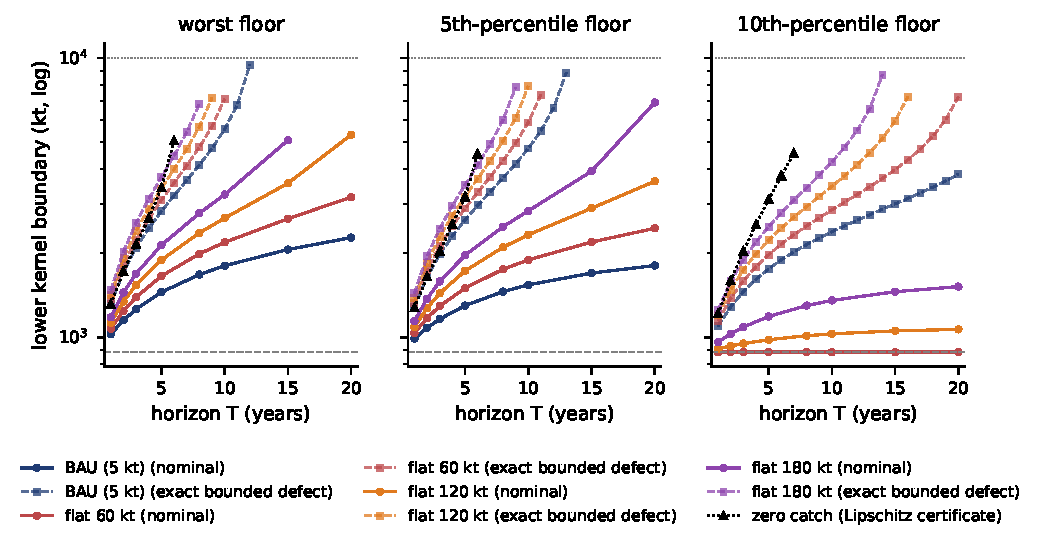
\includegraphics[width=\textwidth]{fig_cod_kernels.pdf}
\caption{Lower boundaries of the cod LRP kernels against the horizon $T$ under the three floors, for BAU, flat 60, 120 and 180 kt. Solid: nominal kernels of the worst-floor map (Theorem~\ref{thm:kernel}); dashed: exact bounded-defect kernels (Theorem~\ref{thm:exact}) with the declared defect $\varepsilon=329\kt$; dotted black: Lipschitz certificate for zero catch. The grey dashed line is the LRP and the dotted line the $10\,000$-kt ceiling at which a kernel becomes empty. Under the 10th-percentile floor the nominal BAU and 60-kt kernels are the whole safe set at every horizon.}
\label{fig:cod-kernels}
\end{figure}


\subsection{Staged rules at the reference point}\label{sec:cod-staged}

The Stage-I rule and the declared cascade take the value 60 kt everywhere on the safe set and differ from the flat 60-kt cap only below the LRP. By Proposition~\ref{prop:stage}(iii) their kernels of the LRP coincide with those of flat 60 kt at every horizon and under every floor, and Table~\ref{tab:cod-kernels} confirms it to the last digit. The cuts to 30, 5 and 0 kt below the LRP protect the lower lines $0.75\,\LRP$ and $0.5\,\LRP$; they contribute nothing to the certification of the LRP itself. The graded rules, which raise catch above the LRP, are \emph{less} protective at $T=5$ (boundaries $1754.3$ and $1715.1$ kt under the worst floor against $1656.7$ kt) because their higher stages are reached above $1.25\,\LRP$; at $T=1$ the 60/90 rule ties flat 60 kt and the 30/60/90 rule, which takes only 30 kt at the LRP, is the more protective ($1047.4$ kt).

The retention test of Section~\ref{sec:frame} therefore fails for both staged rules on the registered family. Clause (a) requires a rule to be at least as protective as BAU at every reading; under the worst and q05 floors the 60-kt rules have strictly higher boundaries than the 5-kt BAU, and under the q10 floor they tie it. Clause (b) is moot. Nothing in the frozen model distinguishes the precautionary-framework Stage-I rule from a flat 60-kt cap at the LRP, and the model says that a flat 60-kt cap is at least as good as the cascade for the LRP at every horizon. The mean supply of the rules on the observed 1983--2007 states is 10.0 kt for S1 and 16.3 kt for the cascade against 5 kt for BAU, with the cut active in 83\% of years (SI Section~S3); supply is not what separates them.

\subsection{Certified horizons under the declared defect}\label{sec:cod-horizon}

The registered certificate inflates the LRP by $r_T=\varepsilon(a^{T}-1)/(a-1)$ with $a=F'(\LRP)=1.1531$ and $\varepsilon=329.0$ kt: $r_1,\dots,r_7=329$, $708$, $1146$, $1650$, $2232$, $2902$, $3675$ kt, growing by $379$ to $773$ kt a year. The certified kernel at horizon $T$ is the nominal $T$-step kernel of $\LRP+r_T$, and it is non-empty exactly as long as the worst-case orbit from the ceiling stays above $\LRP+r_T$ (Theorem~\ref{thm:kernel}(d)); that orbit falls from $10\,000$ kt through $7297$, $6169$, $5493$, $5031$, $4690$, $4425$ and $4211$ kt under BAU and the worst floor, so the certificate holds through $T=6$ and fails at $T=7$ ($r_7=3675$ kt against an orbit at $4211$ kt). Table~\ref{tab:horizons} shows the result for every rule: six years under the worst and q05 floors and seven under q10 for every catch from zero to 150 kt, six for 180 kt, five for 240 kt. Under the registered certificate a manager cannot buy certified years by fishing less: the horizon is a property of the map's expansion at the reference point, which no catch level changes, and the policy-independent bound of Proposition~\ref{prop:finite}(i) is $\lfloor\ln(1+9115\times0.1531/329)/\ln1.1531\rfloor=11$.

\begin{table}[t]
\centering
\caption{Certified horizons under the declared defect: Lipschitz certificate versus exact bounded-defect kernel.}
\label{tab:horizons}
\small
\begin{tabular}{lrrrrrr}
\toprule
System: policy & \multicolumn{2}{c}{worst floor} & \multicolumn{2}{c}{q05 floor} & \multicolumn{2}{c}{q10 floor} \\ & Lip. & exact & Lip. & exact & Lip. & exact \\
\midrule
cod: zero catch & 6 & 12 & 6 & 13 & 7 & 28 \\
cod: BAU (5 kt) & 6 & 12 & 6 & 13 & 7 & 27 \\
cod: flat 60 kt & 6 & 10 & 6 & 11 & 7 & 20 \\
cod: S1 (60 kt above LRP, 0 below) & 6 & 10 & 6 & 11 & 7 & 20 \\
cod: cascade (60/30/5/0) & 6 & 10 & 6 & 11 & 7 & 20 \\
cod: flat 120 kt & 6 & 9 & 6 & 10 & 7 & 16 \\
cod: flat 180 kt & 6 & 8 & 6 & 9 & 6 & 14 \\
cod: flat 240 kt & 5 & 8 & 5 & 8 & 6 & 12 \\
\midrule
Edwards: BAU ($\bar P$) & 3 & 3 & 3 & 3 & 3 & 3 \\
Edwards: flat 90\% & 3 & 3 & 3 & 3 & 3 & 3 \\
Edwards: flat 80\% & 3 & 3 & 3 & 3 & 3 & 3 \\
Edwards: Stage I ($-20\%$ below 660 ft) & 3 & 3 & 3 & 3 & 3 & 3 \\
Edwards: CPM cascade & 3 & 3 & 3 & 3 & 3 & 3 \\
Edwards: zero pumping & 4 & 4 & 5 & 5 & 5 & 5 \\
\bottomrule
\end{tabular}
\par\smallskip\begin{minipage}{0.97\linewidth}\footnotesize Last horizon $T$ (years) at which the certified kernel of the threshold (cod: LRP; Edwards: 618 ft) is non-empty, for the declared uniform defect $\varepsilon$ (cod 329.0 kt, Edwards 15.41 ft) on top of the floor class. `Lip.': the registered Lipschitz-inflation certificate, nominal kernel of $\theta+r_T$ with $r_T=\varepsilon(a^T-1)/(a-1)$ (Proposition~\ref{prop:lip}). `Exact': the exact robust kernel of the bounded-defect class, $W^\varepsilon_{t+1}=\{x: [F(x)-\varepsilon,F(x)+\varepsilon]\subset W^\varepsilon_t\}$ (Theorem~\ref{thm:exact}). For the affine aquifer map the two coincide wherever the backward recursion binds (Proposition~\ref{prop:lip}(ii)); for the expansive cod map the Lipschitz certificate is conservative in horizon and, unlike the exact kernel, is insensitive to the catch level. With the out-of-sample Edwards defect (21.81 ft), positive-pumping rules have a two-year exact horizon and zero pumping retains three years.\end{minipage}
\end{table}


The exact bounded-defect kernel of Theorem~\ref{thm:exact} is less conservative and \emph{is} policy-sensitive. Its boundaries under BAU and the worst floor run $1318$, $1714$, $2089$, $2456$, $2828$, $3219$, $3648$, $4143$ kt at $T=1,\dots,8$ and reach the ceiling at $T=13$. The exact horizons (worst/q05/q10) are 12/13/27 years for BAU, 12/13/28 for zero catch, 10/11/20 for flat 60 kt, 9/10/16 for 120 kt, 8/9/14 for 180 kt and 8/8/12 for 240 kt; Stage I and the cascade share the flat-60 horizons because they take 60 kt at the LRP (SI Section~S4). The reason is Proposition~\ref{prop:lip}(iii): expansion is local to the reference point. The Lipschitz recursion charges $a=1.153$ at every step; the exact recursion propagates the defect through the inverse map evaluated where the boundary actually sits, and at $2500$ kt the slope is already $1$ and at $4000$ kt it is $0.86$. Both certificates are valid; the exact one is the kernel itself. We report the registered figure as the frozen protocol's answer and the exact figure as the sharp one. Neither is indefinite: by Proposition~\ref{prop:finite}(i) an indefinite certificate would need $C+|e|+\varepsilon\le\gmax$, i.e.\ $C\le\Cvac-\varepsilon=215.2-329.0<0$ under the q10 floor and less under the others. With the declared defect no catch level, including the moratorium, is certifiable for ever, and the question for management is the length of the horizon, not its existence.

Finite-duration floors sharpen the harsh classes. If the floor is assumed for $n$ consecutive years and the zero-residual map thereafter, the state needed to absorb it is the $n$-step boundary of Theorem~\ref{thm:kernel}(a): under the q05 floor $1298.7$ kt for five BAU years and $1697.8$ kt for fifteen; $1499.6$ and $2193.4$ kt for the 60-kt rules (SI Section~S5). Five consecutive 5th-percentile years are survivable from about $1.5\,\LRP$; the perpetual version of the same floor is not survivable from anywhere.

\subsection{The stochastic reading}\label{sec:cod-stoch}

The floor classes are worst-case objects. The stochastic layer of the registered campaign asks the complementary question---how often does the LRP hold when the fit residuals are resampled?---with $N=20\,000$ trajectories per cell under three schemes: independent draws, blocks of four consecutive residuals (to keep the two collapse residuals together), and independent draws with 1992 removed. The top block of Table~\ref{tab:cod-unc} gives the 20-year survival from the LRP: $0.903$ for BAU, $0.835$ for 60 kt and $0.647$ for 120 kt under independent draws; $0.852$, $0.807$ and $0.650$ under blocks; $0.954$, $0.917$ and $0.769$ with 1992 removed. An independent re-run of the i.i.d.\ scheme with a different seed reproduces the first row to within $0.002$. The ceiling under independent draws, $0.906$ at zero catch, is arithmetic rather than biology: a draw of the 1992 residual from the LRP is fatal in one step, and if that were the only hazard the ceiling would be $(23/24)^{20}=0.427$; the kernel is larger than that because trajectories climb away from the LRP before the draw occurs. Scanning constant catch from zero, survival crosses $0.9$ at $13.5$ kt under independent draws and never under blocks, and crosses $0.8$ at $81.2$ kt (i.i.d.), $72.3$ kt (blocks) and $105.2$ kt (no 1992); at the constructive bound itself ($92.5$-kt cell) survival is $0.742$, $0.727$ and $0.844$. The stochastic and the worst-case readings agree on the ordering of rules and disagree, as they must, on the meaning of the number: $\Cstar$ is the catch at which the LRP is held against every residual at or above the q10 floor, and at that catch the resampled model loses the LRP within twenty years about one time in four.

\begin{table}[t]
\centering
\caption{Northern cod: stochastic and identification layers around the constructive bound.}
\label{tab:cod-unc}
\small
\resizebox{\textwidth}{!}{%
\begin{tabular}{lrrr}
\toprule
\multicolumn{4}{l}{} \\
\midrule
\multicolumn{4}{l}{\emph{Stochastic layer: 20-year survival from the LRP, $N=20\,000$ trajectories per cell}} \\
scheme & BAU (5 kt) & flat 60 kt & flat 120 kt \\
i.i.d. residuals & 0.903 & 0.835 & 0.647 \\
4-year blocks & 0.852 & 0.806 & 0.650 \\
i.i.d., 1992 removed & 0.954 & 0.917 & 0.769 \\
independent re-run (seed 20261015) & 0.902 & 0.837 & 0.645 \\
catch at which survival crosses 0.9 / 0.8 (kt) & i.i.d.: 13.5 / 81.2 & blocks: none / 72.3 & no-1992: 78.9 / 105.2 \\
\midrule
\multicolumn{4}{l}{\emph{Identification of $C^*=g(\theta)-|e_{q10}|$ (kt)}} \\
source & median & 90\% interval & share $C^*\le 0$ \\
fixed-$K$ residual bootstrap ($B=2000$, archived) & 78.7 & [-69.3, 121.1] & 235/2000 \\
same design, independent seed & 78.8 & [-62.4, 120.3] & 12.5\% \\
joint $(r,K)$ refit ($B=2000$, archived) & 73.7 & [-89.4, 125.7] & 387/2000 \\
\quad conditional on $K\ge 2\theta$ (72.9\% of refits) & 88.1 & [-5.6, 130.6] & 83/1457 \\
profile set in $K$, one-parameter cut (1.195) & -- & [67.9, 95.2] & $K\ge1500$ \\
profile set in $K$, two-parameter cut (1.313) & -- & [51.5, 95.2] & $K\ge1275$ \\
\bottomrule
\end{tabular}
}
\par\smallskip\begin{minipage}{0.97\linewidth}\footnotesize Survival: fraction of trajectories that never fall below the LRP within 20 years when the fitted residuals are resampled (schemes as labelled); the ceiling under i.i.d. resampling is 0.906 because any draw of the 1992 residual ($-329.0$ kt) from the LRP is fatal and $(23/24)^{20}=0.427$ would be the ceiling if the 1992 draw were the only hazard. Bootstraps resample fit residuals along the registered map from the 1983 state with the observed catches and refit $r$ (and $K$ in the joint design); the floor is held at its declared value. Profile sets: $K$ is unidentified from above (the sets run to the top of the 50\,000-kt grid); the SSE at the box edge exceeds the profile minimum by 2.7\%.\end{minipage}
\end{table}


\subsection{Identification}\label{sec:cod-ident}

Because $K$ sits at the edge of its box, the first question a referee asks is whether $\Cstar$ is an artefact of the pin. It is not. The profile in $K$ (closed-form $r$ at each $K$; SI Section~S6, Figure~\ref{fig:cod-ident}a) has its minimum at the top of the 50\,000-kt grid, with the sum of squares at $K=5000$ only $2.7\%$ above it. Under the one-parameter 95\% profile cut ($\mathrm{SSE}/\mathrm{SSE}_{\min}\le1.195$) the set is $K\ge1500$ kt; under the two-parameter joint-region cut ($\le1.313$) it is $K\ge1275$ kt. Over the first set $g(\LRP)$ ranges over $[148.8,176.1]$ kt and $\Cstar$ over $[67.9,95.2]$ kt; over the second $[132.4,176.1]$ and $[51.5,95.2]$ kt. The constant that decides the q10 column is identified even though $K$ is not, because $g(\LRP)=r\LRP(1-\LRP/K)$ is nearly flat in $K$ once $K\gg\LRP$ and the data pin $r(K)$ along the profile. Expansion at the LRP ($F'(\LRP)>1$, i.e.\ $K>2\LRP=1769$ kt) holds throughout both sets except their lowest fringe.

The bootstraps in the lower block of Table~\ref{tab:cod-unc} resample fit residuals along the registered map from the 1983 state with the observed catches and refit. With $K$ held at the box edge the median refit $\Cstar$ is $78.7$ kt with 90\% interval $[-69.3,121.1]$ kt and $235$ of $2000$ refits non-positive; an independent re-run with a different seed gives $78.8$ kt, $[-62.4,120.3]$ kt and $12.5\%$. Re-fitting $K$ jointly, $41.7\%$ of refits pin at 5000 kt, $72.9\%$ are expansive, the median $\Cstar$ is $73.7$ kt with 90\% interval $[-89.4,125.7]$ kt, and conditional on the expansive regime ($K\ge2\LRP$, the regime every result above assumes) the median is $88.1$ kt with interval $[-5.6,130.6]$ kt and $83$ of $1457$ refits non-positive. A positive constructive bound is sampling-stable; its magnitude is not better known than about $\pm40$ kt, and the lower tail is driven by refits in which the two collapse residuals are drawn more than twice. The zero-budget model---the $(r,K)$ pair at which $\Cstar=0$ with $K=5000$, $r=0.1111$---has a sum of squares $1.246$ times the committed fit and $1.279$ times the profile minimum: inside the two-parameter 95\% region, outside the one-parameter profile cut. The data do not exclude a model under which no catch is self-viable at the q10 floor; they make it a 95\% boundary case.

Three further checks are archived and summarised in SI Section~S6. Attributing a share $\lambda$ of residual variance to observation error raises $\Cstar$ from $91.6$ kt ($\lambda=0$) to $112.1$ kt ($\lambda=0.5$) and removes the vacuous class from $\lambda\ge0.2$. The Fox form ($g=rS\ln(K/S)$) refit on the same window gives $\Cstar=79.1$ kt and $\Cvac=111.2$ kt and the same kernel structure; the free Allee refit is a boundary solution and does not define admissible constants, while the declared-$s_0$ Allee row gives $\Cstar=123.3$ kt. Post-moratorium windows (1995--2015, 1995--2007) have small residuals and large $\Cstar$ ($165.7$--$171.4$ and $274.0$ kt): in 1995--2015 the exact minimiser is $K=4316.6$ kt ($\Cstar=165.7$ kt), versus $\Cstar=171.4$ kt at the archived $K=5000$-kt box edge; both windows omit the collapse. The 2024 assessment series (xteNCAM, LRP 276 kt) fitted on 2005--2024 or 1995--2024 pins $K$ at the \emph{lower} edge of the box and gives $\Cstar=-7.7$ and $+8.0$ kt against its own LRP. The certification frame transfers to the new series; the conclusions do not, and the paper makes no claim about the 2024 reference point beyond that observation.

\begin{figure}[t]\centering
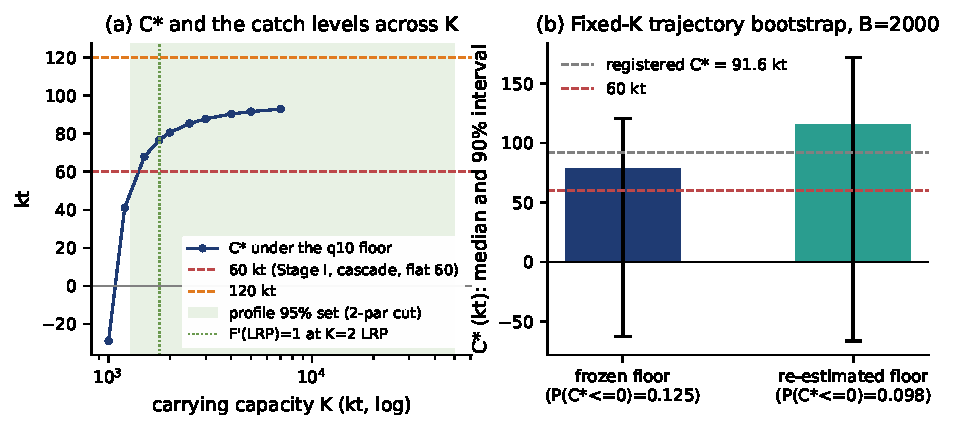
\includegraphics[width=\textwidth]{fig_cod_ident.pdf}
\caption{Identification of the cod verdicts. (a)~$\Cstar(K)=g(\LRP;K,\hat r(K))-|e_{q10}|$ along the profile grid (archived identification campaign), with the 60-kt and 120-kt catch levels, the profile 95\% set (two-parameter cut) and the expansion boundary $K=2\LRP$. The 60-kt rules clear $\Cstar$ for every $K$ in the set; 120 kt clears it for none. (b)~Median and 90\% interval of $\Cstar$ under the fixed-$K$ trajectory bootstrap ($B=2000$, independent seed), with the floor frozen at the registered value and with the floor re-estimated in each replicate.}
\label{fig:cod-ident}
\end{figure}

\section{Edwards Aquifer: the J-17 triggers under an affine recharge--pumping map}\label{sec:edwards}

\subsection{Data, map and declarations}\label{sec:edw-data}

The state is the annual mean elevation $H_t$ of the J-17 index well (TWDB well 6837203, ft above mean sea level), the control is total well pumping $P_t$ and the driver is total recharge $R_t$ (both in $10^3$ acre-ft; \cite{Umphres2025,EAA2023,TWDB}), on a locked 90-year panel 1934--2023 (Figure~\ref{fig:data}b). The map is the one-pool water balance in affine form,
\begin{equation}\label{eq:edw-map}
H_{t+1}-H_t=\alpha+\beta R_{t+1}+\gamma P_{t+1}+\delta H_t+e_{t+1},\qquad a=1+\delta,
\end{equation}
fitted by ordinary least squares on the 56 transitions with destination years 1935--1990: $\alpha=163.49$, $\beta=0.01983$, $\gamma=-0.02844$, $\delta=-0.2539$, so $a=0.7461$ and the map is a contraction. The sign pattern is the physical one (recharge raises, pumping lowers, head decays toward an equilibrium). The fit residuals have standard deviation $5.60$ ft, lag-one autocorrelation $-0.31$ and largest absolute value $15.41$ ft (1971), which is the declared defect. The 33 out-of-sample transitions 1991--2023 have standard deviation $8.40$ ft and largest absolute value $21.81$ ft (2004): the declaration is \emph{exceeded} out of sample, and Section~\ref{sec:edw-horizon} carries both defects. The floor classes are recharge floors from the fit window---the 1956 minimum $43.7$, the 5th percentile $166.5$ and the 10th percentile $179.1$ ($10^3$ acre-ft)---and the reference pumping is the fit-window mean $\Pbar=282.16$. Two thresholds are declared: 618 ft (the physical trigger of the Habitat Conservation Plan) and 660 ft (the Stage-I institutional trigger), with the ceiling at 710 ft. The rule family comprises BAU ($P=\Pbar$), flat caps at 90, 80, 70, 60, 50 and 0\% of $\Pbar$, the Stage-I rule ($-20\%$ below 660 ft) and the four-stage Critical Period Management cascade (cuts of 20, 30, 35 and 40\% below 660, 650, 640 and 630 ft).

\subsection{Attractors, kernels and the securability of the two triggers}\label{sec:edw-kernels}

By Corollary~\ref{cor:edw} every constant-pumping question is decided by the worst-floor attractor $\Hstar=(\alpha+\beta\underline R+\gamma P)/(1-a)$, and by Proposition~\ref{prop:stage} a staged rule is decided by the attractor of the stage that contains it. Table~\ref{tab:edw} lists them. Under the 1956 recharge floor BAU settles at $615.7$ ft, below 618; every cut of 10\% or more settles above it (flat 90\%: $618.9$ ft), and the smallest flat cut that secures 618 ft is $1-\rho^{*}=7.2\%$ of $\Pbar$ by Theorem~\ref{thm:margin}---a pumping level of $261.8$, which is $31.5\%$ below the 1991--2023 mean of $382.1$. The Stage-I rule settles at the flat-80\% attractor ($622.0$ ft) because the head it converges to lies below 660 ft where its cut is active, and the cascade settles at the flat-60\% attractor ($628.4$ ft) in its 40\% stage. Under the 5th- and 10th-percentile floors every rule including BAU clears 618 ft.

\begin{table}[t]
\centering
\caption{Edwards Aquifer: attractors, kernels and open-loop supply by policy.}
\label{tab:edw}
\small
\resizebox{\textwidth}{!}{%
\begin{tabular}{lrrrllrr}
\toprule
Policy & \multicolumn{3}{c}{attractor $H^*$ (ft)} & 618-ft kernel & 660-ft $b_1/b_2/b_3$ & supply & cut active \\ & worst & q05 & q10 & (worst floor) & (worst floor) & &  \\
\midrule
BAU ($\bar P$) & 615.7 & 625.3 & 626.3 & empty from $T=13$ & 675.1 / 695.3 / $\emptyset$ & 282.2 & 0\% \\
flat 90\% & 618.9 & 628.5 & 629.5 & whole safe set & 674.0 / 692.8 / $\emptyset$ & 253.9 & 100\% \\
flat 80\% & 622.0 & 631.6 & 632.6 & whole safe set & 672.9 / 690.2 / $\emptyset$ & 225.7 & 100\% \\
flat 70\% & 625.2 & 634.8 & 635.8 & whole safe set & 671.8 / 687.7 / 709.0 & 197.5 & 100\% \\
flat 60\% & 628.4 & 638.0 & 638.9 & whole safe set & 670.8 / 685.2 / 704.5 & 169.3 & 100\% \\
flat 50\% & 631.5 & 641.1 & 642.1 & whole safe set & 669.7 / 682.7 / 700.1 & 141.1 & 100\% \\
zero pumping & 647.3 & 656.9 & 657.9 & whole safe set & 664.3 / 670.1 / 677.8 & 0.0 & 100\% \\
Stage I ($-20\%$ below 660 ft) & 622.0 & 631.6 & 632.6 & whole safe set & 675.1 / 695.3 / $\emptyset$ & 262.4 & 35\% \\
CPM cascade & 628.4 & 636.4 & 637.4 & whole safe set & 675.1 / 695.3 / $\emptyset$ & 254.9 & 35\% \\
\bottomrule
\end{tabular}
}
\par\smallskip\begin{minipage}{0.97\linewidth}\footnotesize Attractor $H^*=(\alpha+\beta F+\gamma P)/(1-a)$ of the stage that contains it (self-consistent fixed point of the closed loop) under the three recharge floors $F$. 618-ft kernel under the worst floor: whole safe set iff $H^*\ge 618$ (Corollary~\ref{cor:edw}); otherwise empty beyond $T_{\mathrm{empty}}$. 660-ft column: lower boundary at $T=1/2/3$ under the worst floor; zero pumping is the only rule whose 660-ft kernel survives to $T=3$, and none survives $T=\infty$ because $H^*_0=(\alpha+\beta F)/(1-a)=647.3$ ft $<660$ (Theorem~\ref{thm:margin}). Supply: mean prescribed pumping on the observed 1934--1990 heads ($10^3$ acre-ft yr$^{-1}$) and share of years with the cut active.\end{minipage}
\end{table}


The 618-ft kernels follow. For every cut policy they are the whole safe set at every horizon under every floor. For BAU under the worst floor they are the empty-in-finite-time case of Theorem~\ref{thm:kernel}(d): $b_T=\Hstar+(618-\Hstar)/a^{T}$ runs $618.8$, $619.8$, $621.2$, $625.6$, $639.5$, $658.4$ and $692.4$ ft at $T=1,2,3,5,8,10,12$ and passes the 710-ft ceiling at $T=13$, in agreement with the closed form $\Tempty=\lfloor12.70\rfloor+1$. A manager who pumps the historical mean through a repeat of 1956 recharge can keep J-17 above 618 ft for twelve years only by starting above $692$ ft, which is above the highest annual mean in the ninety-year record ($692.0$ ft). Finite-duration floors (SI Section~S10) say the same with less drama: five consecutive 1956 years under BAU are absorbed from $625.6$ ft, ten from $658.4$ ft, fifteen from nowhere; every cut policy absorbs any run.

The 660-ft trigger is a different object. Theorem~\ref{thm:margin} asks whether the zero-pumping attractor clears it: $\Hstar_0=(\alpha+\beta\underline R)/(1-a)=647.3$, $656.9$ and $657.9$ ft under the three floors, short of 660 by $12.7$, $3.1$ and $2.1$ ft. No admissible rule can hold 660 ft from itself under any declared floor; the kernels are empty in finite time for every rule, at $T=3$ for BAU, the Stage-I rule and the cascade (whose 660-ft kernels coincide, since all three pump $\Pbar$ at and above 660 ft), at $T=6$ for zero pumping (SI Section~S8). The institutional trigger is a line the aquifer is managed \emph{around}, not a line that can be certified; the physical trigger is one that can.

\begin{figure}[t]\centering
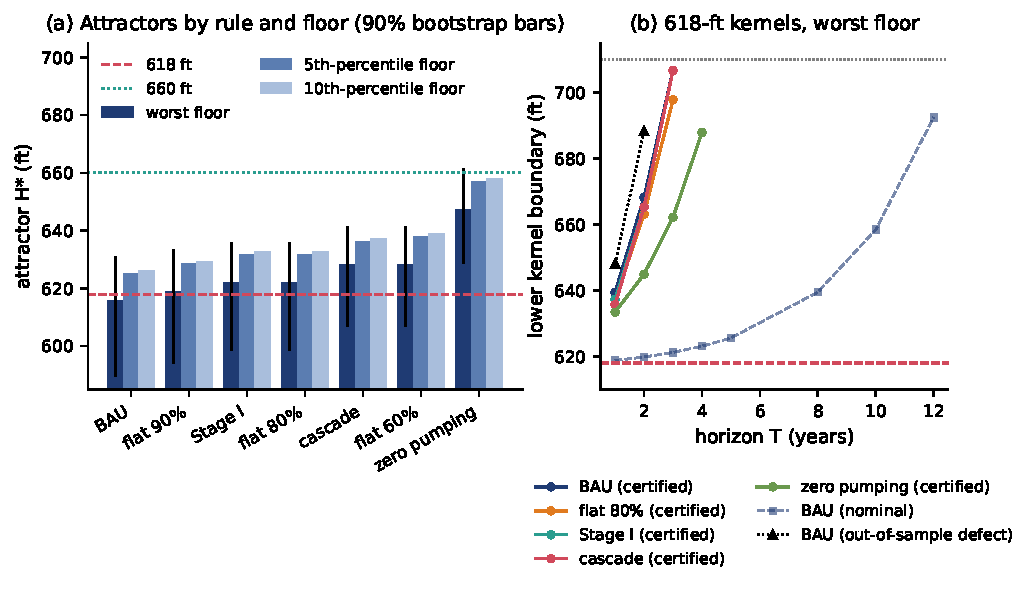
\includegraphics[width=\textwidth]{fig_edw_kernels.pdf}
\caption{Edwards Aquifer kernels. (a)~Worst-floor attractors $\Hstar$ of the rule family under the three recharge floors (Corollary~\ref{cor:edw}, Proposition~\ref{prop:stage}), with 90\% intervals from the archived residual bootstrap of the fit; the staged rules inherit the interval of the flat cap of their stage at the attractor. (b)~Lower boundaries of the 618-ft kernels under the 1956 floor: Lipschitz-certified kernels with the declared defect for five rules (solid), the nominal BAU kernel (dashed), and the exact bounded-defect BAU kernel under the out-of-sample defect of $21.8\ft$ (dotted). The dotted grey line is the 710-ft ceiling.}
\label{fig:edw-kernels}
\end{figure}


\subsection{Supply and retention}\label{sec:edw-supply}

Protection ties are broken by supply. On the observed 1934--1990 heads the Stage-I rule's cut is active in 20 of 57 years ($35\%$) and it prescribes a mean of $262.36$, against $253.94$ for the flat 90\% cap and $225.73$ for flat 80\%; the observed heads lie below 660, 650, 640 and 630 ft in 20, 12, 5 and 1 of 57 years and the cascade prescribes $254.93$, against $169.29$ for the flat 60\% cap whose protection it matches. Clause (a) of the retention rule holds for both staged rules at every reading (they are never less protective than BAU), and clause (b) holds at the 618-ft worst-floor reading: the Stage-I rule supplies $3.3\%$ more than the least protective flat cap that matches it at the nominal level (flat 90\%) and $16.2\%$ more than the one that matches it at the certified level (flat 80\%); the cascade supplies $50.6\%$ more than flat 60\% and $0.4\%$ more than flat 90\%. Both staged rules are retained. On the 33 out-of-sample heads the cut is active in 11 years ($33\%$) and the supplies are $263.35$ and $258.22$ ($10^3$ acre-ft yr$^{-1}$).

Open-loop supply evaluates a rule on heads it did not produce. The closed-loop replay (model driven by observed recharge, pumping by the rule, from the observed 1934 head; Figure~\ref{fig:edw-replay}a) corrects for this: the Stage-I rule supplies $258.98$ with the cut active in $41\%$ of years, $2.0\%$ more than flat 90\% and $14.7\%$ more than flat 80\%; the cascade supplies $254.70$, $50.4\%$ more than flat 60\%. The retention conclusions survive the correction. Out of sample (from the 1990 head through the 33 transitions to 2023; Figure~\ref{fig:edw-replay}b) the Stage-I rule supplies $268.48$ with the cut active in $24\%$ of years and ends 2023 at $643.3$ ft against an observed $635.7$ ft, the observed series having been pumped at a mean of $382$ rather than $282$. Under a recharge pinned at the 1956 floor for 57 years the staged rules spend most of the time in their deepest stage and their supply advantage shrinks to the stage margin ($226.7$ against $225.7$ for Stage I and flat 80\%; $174.5$ against $169.3$ for the cascade and flat 60\%; SI Section~S10).

\subsection{Certified horizons and the bounded-defect audit}\label{sec:edw-horizon}

With $a<1$ the Lipschitz accumulation saturates: $r_T=\varepsilon(1-a^{T})/(1-a)$ runs $15.41$, $26.91$, $35.49$, $41.89$, $46.66$ ft at $T=1,\dots,5$ and tends to $r_\infty=60.70$ ft. The certified 618-ft kernel at horizon $T$ is the nominal kernel of $618+r_T$, and by Corollary~\ref{cor:edw} its boundary is $\Hstar+(618+r_T-\Hstar)/a^{T}$ whenever that exceeds $618+r_T$. For BAU under the worst floor the certified boundaries are $639.4$, $668.2$ and $706.7$ ft at $T=1,2,3$ and the kernel is empty at $T=4$; the Stage-I rule and the cascade reach the same $706.7$ ft at $T=3$ (their attractors differ, but the $1/a^{T}$ factor dominates), flat 80\% reaches $697.8$ ft, and only zero pumping survives to $T=4$ ($687.9$ ft) under the worst floor; under the two quantile floors the 50\% and 60\% caps reach $T=4$ and zero pumping $T=5$. The registered Lipschitz certificate for 660 ft fails at $T=2$ for every rule. Table~\ref{tab:horizons} collects the horizons and Figure~\ref{fig:edw-kernels} draws the boundaries.

Proposition~\ref{prop:lip}(ii) says that for an affine closed-loop map the exact bounded-defect kernel of Theorem~\ref{thm:exact} coincides with the Lipschitz certificate wherever the backward recursion binds. The BAU boundaries are $639.43$, $668.16$, and $706.66$ ft, identical to the certificate, with the kernel empty at $T=4$; the positive flat caps likewise coincide at every reported horizon, as does zero pumping from $T=3$ onward. The departures are of two kinds and neither lengthens a horizon. For zero pumping at $T=1,2$ the certificate's inflation of the initial state is the binding constraint and the exact kernel is larger ($628.7$ and $643.0$ against $633.4$ and $644.9$ ft). For the two staged rules the closed-loop map is piecewise affine rather than affine, because a perturbed head can cross 660 ft and engage the cut, and the exact kernel is larger by $2$--$7$ ft at $T=2,3$ (Stage I $702.8$ against $706.7$ ft at $T=3$; cascade $663.1$ and $699.9$ against $665.3$ and $706.7$ ft) while still emptying at $T=4$. These departures sharpen boundary locations but add no certified year: for positive pumping the three-year horizon is a property of the declared class, not a looseness in the Lipschitz method. Proposition~\ref{prop:finite}(ii) makes the point structurally: an indefinite certificate requires an attractor at least $r_\infty=60.7$ ft above the threshold, i.e.\ $678.7$ ft, and the highest attractor in the family is $657.9$ ft (zero pumping, q10 floor).

Because the out-of-sample residual exceeds the declaration, the audit of Table~\ref{tab:edw-unc} asks how large a uniform defect the 618-ft kernel can carry at each horizon. The supremum at $T=3$ is $16.01$ ft for BAU, $16.71$ ft for Stage I, $17.23$ ft for the cascade, $17.62$ ft for flat 80\% and $24.04$ ft for zero pumping; at $T=4$ it is $9.91$--$11.60$ ft for the pumping rules and $17.93$ ft for zero pumping. The declared $15.41$ ft clears every $T=3$ supremum and no $T=4$ supremum except zero pumping's; the out-of-sample $21.81$ ft clears only zero pumping's at $T=3$: every positive-pumping rule's exact kernel is empty at $T=3$ (BAU boundaries $648.0$ and $688.2$ ft at $T=1,2$), while zero pumping's kernel is empty at $T=4$. The out-of-sample defect accumulates to $r_\infty=85.9$ ft. For positive-pumping rules the certified horizon is three years on the declared defect and two on the audited one; zero pumping adds one year in each case (four and three years, respectively).

\begin{table}[t]
\centering
\caption{Edwards Aquifer: supply, protection and the bounded-defect audit.}
\label{tab:edw-unc}
\small
\setlength{\tabcolsep}{4pt}
\begin{tabular}{lrrrr}
\toprule
\multicolumn{5}{l}{\emph{Mean annual supply $P$ ($10^3$ acre-ft yr$^{-1}$) and $P(H^*\ge618)$}} \\
\midrule
policy & \shortstack{open loop\\1934--90} & \shortstack{closed loop\\fit 1934--90} & \shortstack{closed loop OOS\\1991--2023} & \shortstack{$P(H^*\ge618)$\\archived / rerun} \\
\midrule
BAU ($\bar P$) & 282.16 & 282.16 (0\%) & 282.16 (0\%) & 0.41 / 0.40 \\
flat 90\% & 253.94 & 253.94 (100\%) & 253.94 (100\%) & 0.53 / 0.52 \\
flat 80\% & 225.73 & 225.73 (100\%) & 225.73 (100\%) & 0.65 / 0.64 \\
flat 60\% & 169.29 & 169.29 (100\%) & 169.29 (100\%) & 0.83 / 0.82 \\
zero pumping & 0.00 & 0.00 (100\%) & 0.00 (100\%) & 0.99 / 0.99 \\
Stage I ($-20\%$ below 660 ft) & 262.36 & 258.98 (41\%) & 268.48 (24\%) & 0.65 / -- \\
CPM cascade & 254.93 & 254.70 (41\%) & 265.06 (24\%) & 0.83 / -- \\
\midrule
\multicolumn{5}{l}{\emph{Exact-kernel supremum defect $\bar\varepsilon_T$ (ft) by horizon}} \\
\midrule
policy & $T=2$ & $T=3$ & $T=4$ & $T=5$ \\
\midrule
BAU ($\bar P$) & 28.75 & 16.01 & 9.91 & 6.44 \\
flat 90\% & 29.55 & 16.82 & 10.71 & 7.25 \\
flat 80\% & 30.36 & 17.62 & 11.51 & 8.05 \\
Stage I ($-20\%$ below 660 ft) & 29.67 & 16.71 & 10.94 & 7.67 \\
CPM cascade & 29.67 & 17.23 & 11.60 & 8.49 \\
zero pumping & 36.77 & 24.04 & 17.93 & 14.47 \\
\bottomrule
\end{tabular}
\par\smallskip\begin{minipage}{0.97\linewidth}\footnotesize Closed-loop replays use observed recharge and rule-based pumping, starting from 1934 (fit) or 1990 (out of sample); percentages in parentheses are years with the cut active. $P(H^*\ge618)$ is the share of 5,000 bootstrap refits whose worst-floor attractor clears 618 ft (archived / independent seeds 20260905 / 20261015). At the declared 15.41-ft defect, every rule certifies three years and only zero pumping lasts four; at the out-of-sample 21.81-ft defect, only zero pumping certifies three years.\end{minipage}
\end{table}


\subsection{Replays and the stochastic reading}\label{sec:edw-stoch}

The 1950s drought is the only episode in the record that reached the physical trigger's neighbourhood: J-17 averaged $623.15$ ft in 1956 (daily minimum $612.51$ ft). Replaying 1951--1956 from the observed 1950 head with actual recharge and each rule's pumping, the model reaches $629.7$ ft under BAU, $632.3$ under flat 90\%, $634.9$ under Stage I and $637.1$ ft under the cascade, all above 618; with the actual (larger) pumping of the 1950s the model reaches $631.2$ ft against the observed $623.2$, a bias of $8.1$ ft that is within the declared defect and in the unsafe direction. Under the fit-window record the staged rules keep the model above $632.9$ and $636.2$ ft; under 1991--2023 recharge all rules end 2023 between $639$ and $671$ ft (SI Section~S10).

The stochastic reading resamples fit residuals, refits \eqref{eq:edw-map} 5000 times and asks how often the worst-floor attractor clears 618 ft: $0.41$ for BAU, $0.53$ for flat 90\%, $0.65$ for flat 80\% and Stage I, $0.83$ for flat 60\% and the cascade, $0.99$ for zero pumping, with a bootstrap standard deviation of $10$--$13$ ft on every attractor; an independent re-run with a different seed reproduces each probability to within $0.012$ (SI Section~S11). The flat-90\% minus BAU attractor gap, $3.2$ ft at the point estimate, has a 90\% bootstrap interval of $[1.9,5.1]$ ft and is positive in every replicate (minimum $0.5$ ft), because $\gamma<0$ in every refit. The ordering of the rules is sampling-stable; the certification of 618 ft by a 7.2\% cut is a statement about the registered fit, and at the fit's own sampling uncertainty it is a coin toss for BAU and a two-to-one bet for the Stage-I rule.

\begin{figure}[t]\centering
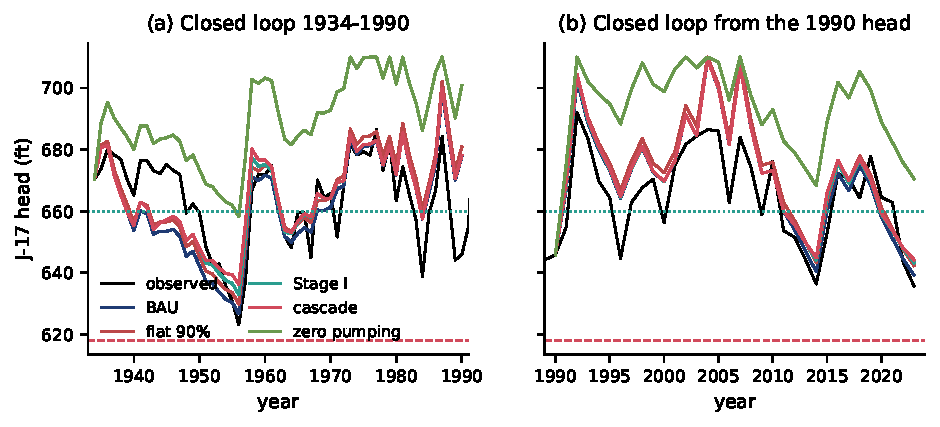
\includegraphics[width=\textwidth]{fig_edw_replay.pdf}
\caption{Closed-loop replays of the Edwards map (observed recharge, pumping prescribed by the rule from the model head, 710-ft ceiling). (a)~From the observed 1934 head through 1990; (b)~from the observed 1990 head through 2023. The observed series was pumped at a mean of $282$ ($10^3$ acre-ft) before 1991 and $382$ after; the replays pump $\Pbar=282$ or the rule's fraction of it.}
\label{fig:edw-replay}
\end{figure}

\section{What the two systems establish together}\label{sec:synthesis}

The two applications share no hydrology, no biology and no institution; they share a frame, a protocol and a verifier. Table~\ref{tab:resolved} lists every question the frame was asked, with the answer and the clause of Section~\ref{sec:frame} that supplies it. Three results are joint.

\begin{table}[t]
\centering
\caption{What the frozen protocols resolve, and what they do not, in the two systems.}
\label{tab:resolved}
\small
\begin{tabular}{p{0.27\textwidth}p{0.32\textwidth}p{0.32\textwidth}}
\toprule
Question & Northern cod & Edwards Aquifer \\
\midrule
Is the reference point self-viable under some constant control? & yes under q10 ($C^*=91.6$ kt); no under q05/worst ($C^*<0$) & yes at 618 ft (any cut $\ge 7.2\%$); no at 660 ft under any floor ($H^*_0=647.3$--657.9 ft) \\
Is any non-empty $T=\infty$ kernel available? & q10: for $C\le C_{\mathrm{vac}}=215.2$ kt; q05: $C\le 8.7$ kt; worst: none & 618 ft: yes for every cut $\ge 7.2\%$; 660 ft: none \\
Does a staged rule beat the flat cap it coincides with at the threshold? & no (S1, cascade $\equiv$ flat 60 kt on the safe set) & no in protection; yes in supply (S1 $+3.3\%$ over flat 90\%, CPM $+50.6\%$ over flat 60\%) \\
Horizon certified under the declared defect (exact kernel) & 8--13 yr (worst/q05), 12--28 yr (q10); Lipschitz: 5--7 yr & 3 yr positive-pumping (4 zero); 2 yr OOS positive-pumping (3 zero) \\
Is the horizon policy-sensitive? & exact: yes (zero catch 12 vs 240 kt 8 yr, worst floor); Lipschitz: no & weakly (3 vs 4 yr) \\
What sets the horizon? & local expansion at the LRP, $F'(\theta)=1.153$ & defect-to-contraction ratio $\varepsilon/(1-a)=60.7$ ft against a 92-ft band to the ceiling \\
Is the key constant identified? & $g(\theta)$ and $C^*$ yes (profile), $K$ no & $a$, $H^*$ yes (bootstrap SD 10--13 ft on $H^*$) \\
Stochastic (non-worst-case) reading & 20-yr survival from the LRP 0.90 (BAU) to 0.65 (120 kt) & $P(H^*\ge618)$: 0.41 (BAU), 0.53 (flat 90\%), 0.65 (S1), 0.99 (zero) \\
\bottomrule
\end{tabular}
\end{table}


\paragraph{Protection and supply are one budget at the threshold.}
At a threshold $\theta$ the kernel of a constant-control rule is decided by the sign of $F(\theta,u)-\theta$ under the worst floor; by Proposition~\ref{prop:stage} a staged rule is decided by its stage at $\theta$. Every rule therefore has one number at $\theta$ and a one-dimensional margin, $\Cstar-C(\theta)$ for the stock and $\Hstar(P(\theta))-\theta$ for the aquifer. A reactive rule cannot out-supply, at the threshold, the flat rule it matches there; where it can out-supply is away from the threshold, and that is where the retention rule looks. For cod the Stage-I rule supplies $10.0\kt$ on the observed states against the flat 60-kt cap's 60, and the two are equally protective: it fails clause (b) and is not retained. For the aquifer the Stage-I rule supplies $3.3\%$ more than flat 90\% on the observed heads at equal nominal protection and $16.2\%$ more than flat 80\% at equal certified protection, and is retained. The rule is the same; the verdicts differ because the observed states of the two systems sit on different sides of the stage boundaries.

\paragraph{Certification has a horizon, and the map sets it.}
The certified horizon of the two systems is set by different features of the fitted map and the declared defect. The cod map is expansive at the LRP ($F'(\theta)=1.153$ under the fitted $K$), so the Lipschitz error grows geometrically and its horizon is six years under the worst/q05 floors and seven under q10 for catches up to 150 kt; the exact bounded-defect kernel extends this to 8--13 years under the two harsher floors and 12--28 under q10, with catch-sensitive horizons (Figure~\ref{fig:horizons}). The aquifer map is contractive ($a=0.746$) and the error saturates at $r_\infty=60.7\ft$. At 618 ft the declared-defect horizon is three years for positive-pumping rules and four at zero pumping; with the out-of-sample defect the horizons are two and three. The exact kernel matches the Lipschitz boundary for positive constant-pumping rules wherever the backward recursion binds, while zero pumping at $T=1,2$ and the staged rules depart locally without changing a horizon (Proposition~\ref{prop:lip}(ii)). Thus the cod Lipschitz result is conservative relative to the exact recursion, whereas the aquifer's positive-pumping horizon is class-limited under the frozen protocol. The mechanisms of boundary departure also differ: curvature lowers the cod boundary away from the threshold; in the aquifer, the inflated initial-state constraint binds at zero pumping and stage crossings make the staged maps piecewise affine.

\begin{figure}[t]\centering
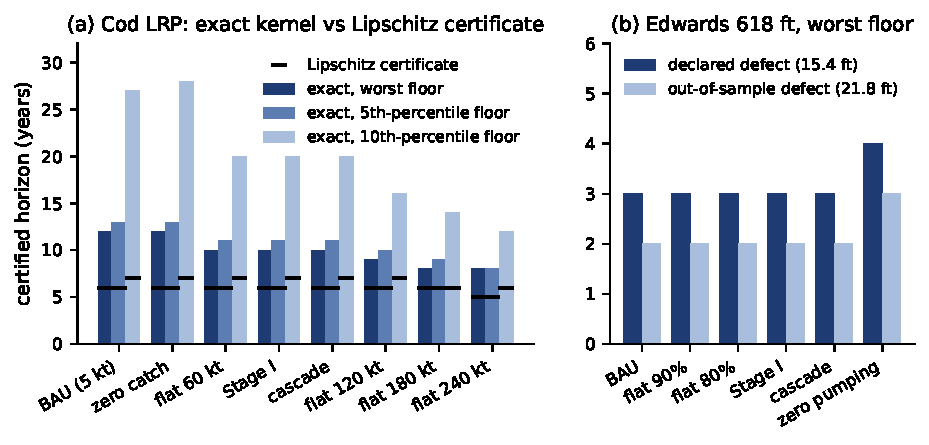
\includegraphics[width=\textwidth]{fig_horizons.pdf}
\caption{Certified horizons. (a)~Cod LRP: last non-empty horizon of the exact bounded-defect kernel under the three floors (bars) and of the Lipschitz certificate (black ticks; for the staged rules the certificate of their 60-kt stage at the LRP). (b)~Edwards 618-ft trigger under the 1956 floor: last non-empty horizon of the exact bounded-defect kernel with the declared defect ($15.4\ft$) and with the out-of-sample defect ($21.8\ft$); the Lipschitz certificate coincides with the exact kernel wherever the backward recursion binds (Proposition~\ref{prop:lip}(ii)); the zero-pumping and staged-rule boundary departures are described in Section~\ref{sec:edw-horizon} and do not change the horizons.}
\label{fig:horizons}
\end{figure}


\paragraph{Thresholds can be unsecurable, and the frame says which.}
Theorem~\ref{thm:margin} reduces securability to one comparison per floor. The cod LRP is secured by any constant catch below $\Cstar$ under every floor; the Edwards 618-ft trigger is secured by any cut of at least $7.2\%$ under the worst floor and by BAU under the two quantile floors; the Edwards 660-ft trigger is secured by nothing, under any declared floor, because the zero-pumping attractor falls short of it by $2.1$--$12.7\ft$. A test that asks only whether a threshold is breached in simulation reports the 660-ft line as frequently crossed and recovered; the frame reports that no admissible rule can be credited with its recovery, which is the operational distinction between a line that is managed \emph{to} and a line that is managed \emph{around}.

\paragraph{Cadence.}
The certified horizons bound the re-certification interval. With a three-year horizon on the declared defect and two on the audited one, the aquifer's registered map should be refitted and the kernels recomputed at least every two years; the cod exact horizon of eight to thirteen years under the harsher floors, read against the six-year review cycle of the International Whaling Commission's management procedures and the one-to-three-year stock-assessment cadence of most North American groundfish, says that the present cadence is inside the certificate for cod and outside it for the aquifer under BAU. Both protocols were frozen on 2026-08-26, before any kernel, boundary, replay or retention score was computed, and both report negative results; a frame that returned only positive verdicts would be advocacy.

\section{Discussion}\label{sec:discussion}

\paragraph{What a certificate is and is not.}
A certified kernel is a statement about a declared class: a registered map, a floor class, a bounded defect and a horizon. It is not a prediction of the trajectory and it is not a probability. The stochastic readings of Sections~\ref{sec:cod-stoch} and~\ref{sec:edw-stoch} are reported beside the kernels so that a reader can see what the two kinds of statement cost: the i.i.d.\ bootstrap survival of the cod LRP under BAU is $0.90$ over twenty years with a ceiling of $0.906$ set by the two collapse residuals, and the frozen-floor bootstrap of $\Cstar$ has $12.5\%$ of its mass at or below zero; the attractor bootstrap puts BAU at the 618-ft trigger at $0.41$. None of these numbers is the kernel and none contradicts it. The kernel says what holds for every sequence in the class; the bootstrap says how often it holds for the sequences the record generates.

\paragraph{The declared defect.}
One audit exceeds its declaration out of sample and the other does not. The cod out-of-sample residuals (2008--2015) are small, with maximum $46.7\kt$, and the declaration of $329\kt$ is conservative by a factor of seven for the post-moratorium regime; the Edwards out-of-sample maximum of $21.8\ft$ exceeds the declared $15.4\ft$; the positive-pumping horizon falls from three years to two, while zero pumping retains three. We keep the declarations as registered and report the audited horizons beside them, because the alternative---redeclaring the defect after seeing the data it is meant to bound---is the practice the protocol exists to prevent. Table~\ref{tab:edw-unc} shows what redeclaration would cost: the supremum defect the three-year aquifer kernel can carry is $16.0$--$17.6\ft$ for the pumping rules ($24.0\ft$ at zero pumping), so a declaration at the out-of-sample maximum leaves only zero pumping certified through $T=3$; even zero pumping fails at $T=4$.

\paragraph{Where the cod verdict is fragile.}
The cod negatives are fragile in one direction and robust in the other. In the fragile direction, the vacuous class under the worst floor ($\Cvac<0$: no state is one-step safe at the 1992 residual) disappears once a share $\lambda\ge0.2$ of the residual variance is attributed to observation error, under a window that starts after the moratorium ($\Cstar=165.7\kt$ for 1995--2015), under the Fox form ($\Cstar=79.1\kt$) and under the 2024 assessment's lower reference point ($\Cstar=-7.7\kt$ at 2005--2024, $+8.0\kt$ at 1995--2024). In the robust direction, the no-dominance verdict for the Stage-I rule does not depend on $K$ (Section~\ref{sec:cod-ident}), on the floor, on the form or on the window, because it is a comparison of two rules that pump the same catch at the LRP. We regard the second kind of result as the paper's contribution to the cod case and the first kind as its honest scope.

\paragraph{Where the aquifer verdict is fragile.}
The Edwards certificate at 618 ft is a statement about a three-parameter affine map with a worst recharge floor taken from the fit window. The map omits spring discharge, the storage nonlinearity of the karst and the spatial structure of pumping; its out-of-sample residual is larger than its fit residual; and its 1950s replay reproduces the drought minimum with an $8\ft$ bias in the unsafe direction. The attractor ordering of the rules survives all of this because it depends only on the sign of $\gamma$, which is negative in every one of 5000 bootstrap refits (the flat-90\% minus BAU gap is positive in all of them, with minimum $0.5\ft$); the location of the BAU attractor relative to 618 ft, a difference of $2.3\ft$ against a bootstrap standard deviation of $13\ft$, does not, and the unsecurability of 660 ft, a shortfall of $2.1$--$12.7\ft$ against a standard deviation of $10\ft$ on the zero-pumping attractor, is a statement about the registered fit rather than about the aquifer. A reader who wants a finer resolution should fit a finer map; the frame will certify it on the same terms.

\paragraph{The retention rule as a design instrument.}
Clause (b) of the retention rule is a supply comparison at equal protection, and it is the only place in the frame where a staged rule can earn its place. The two systems show the two outcomes: where the observed states are mostly above the stage boundaries (the aquifer, 65\% of years above 660 ft), a staged rule banks supply in the unconstrained years and is retained; where they are mostly below (cod, 83\% of the fit-window years below the LRP, where the staged rules take little or nothing), the staged rule supplies less than the flat cap it matches in protection and is not. A manager designing a staged rule can read the rule's prospects off the empirical distribution of the state relative to its boundaries before any kernel is computed.

\paragraph{Limits of the one-dimensional setting.}
Everything above uses that the state is a scalar and the safe set an interval, which makes the kernels half-lines and the exact bounded-defect recursion a one-dimensional dynamic programme. The frame extends to monotone maps on ordered state spaces without change in the statements and with the kernels becoming upper sets; the exact recursion becomes a robust dynamic programme on a grid and loses the closed forms. The staged-rule proposition and the securability theorem are the two results that depend most on dimension one, through the fixed-point structure of Theorem~\ref{thm:kernel}; their analogues in higher dimension are conjectures we do not make here.

\section{Verification}\label{sec:verification}

Every number in this paper is produced by one script, \texttt{p09\_core.py}, from the two locked panels and the registered constants, and every table is generated from its output; no number is typed by hand. The script re-derives the cod fit, the Edwards fit, the floors, the kernels of Theorem~\ref{thm:kernel} by direct backward recursion on the declared ceilings, the exact bounded-defect kernels of Theorem~\ref{thm:exact}, the Lipschitz certificates, the horizons, the supplies, the replays and the bootstraps, and then compares $926$ of its outputs against the archived campaign results of the registered protocol (the family, structure, cadence, identification, depensation and elevation campaigns, and the audit bootstrap), which were produced by different code in 2026-08 and are shipped in the source folder. All $926$ comparisons pass at the tolerances stated in the script (kernel boundaries to $0.15\kt$ and $0.05\ft$, probabilities to $0.02$, bootstrap quantiles to $3\kt$). The archived campaign scripts were also re-executed on the locked panels during preparation of this edition and reproduced their own result files.

Three classes of result are new to this edition and have no archived counterpart: the exact bounded-defect kernels (Section~\ref{sec:cod-horizon}, SI Section~S4), the bounded-error suprema of Table~\ref{tab:edw-unc} at the quantile floors and out-of-sample defect, and the Lipschitz-versus-exact identity of Proposition~\ref{prop:lip}(ii). For these the script checks the closed forms of Section~\ref{sec:frame} against the recursion (the affine $b_T$ and $\Tempty$ of Corollary~\ref{cor:edw}, the proportional-rule thresholds of Corollary~\ref{cor:cod}, the stage reduction of Proposition~\ref{prop:stage}, the identity of Proposition~\ref{prop:lip}(ii) at every binding horizon of every constant-pumping rule, and the monotonicity of the exact kernels in $T$, in the catch and in the defect), and the verifier records the identity's departures for zero pumping and for the staged rules (Section~\ref{sec:edw-horizon}). The stochastic and bootstrap readings are re-run with seeds different from the archive's (cod $20261015$; Edwards $20261015$) and agree with the archived values to the tolerances reported in Sections~\ref{sec:cod-stoch} and~\ref{sec:edw-stoch}.

The shipped verifier \path{paper09_cod_certification_v44_verification.py} runs the core, regenerates the tables and figures, and checks \nchecks{} statements of the manuscript against the regenerated output (every number quoted in the abstract, the theorems' numerical instances, every entry of Tables~\ref{tab:inputs}--\ref{tab:resolved}, the figure data, and the claims of Section~\ref{sec:synthesis}); it exits with a non-zero status on any failure and writes its report to \path{paper09_cod_certification_v44_verification_output.txt}. The verifier, the core, the table generator, the figure script, the locked panels, the archived campaign results and the frozen protocols are in the source folder \path{paper09_cod_certification_v44_src/}; its \texttt{README} gives the commands that rebuild everything from the panels. The two protocols are reproduced verbatim in SI Section~S13 with their freeze dates.

\section{Related work}\label{sec:related}

\paragraph{Viability kernels and robust invariance.}
The viability kernel is Aubin's \cite{Aubin1991}; its discrete-time robust form, the largest set from which a target tube can be held against a bounded adversary, is the minimax reachability problem of Bertsekas and Rhodes \cite{BertsekasRhodes1971,Bertsekas1972}, surveyed with the invariance literature by Blanchini \cite{Blanchini1999}. Saint-Pierre's algorithm \cite{SaintPierre1994} computes kernels by backward set recursion on a grid, which is the computation we specialise to one dimension, where the sets are intervals and the recursion has closed forms. The exact bounded-defect kernel of Theorem~\ref{thm:exact} is the robust kernel of the map perturbed by an additive bounded disturbance; its relation to the Lipschitz inflation, Proposition~\ref{prop:lip}, is the standard inner-approximation argument, with equality for affine maps wherever the backward recursion binds. Regnier and De Lara \cite{RegnierDeLara2015} develop robust viability for a harvested ecosystem under set-valued uncertainty and are the closest antecedent for the floor-class formulation; De Lara and Doyen's monograph \cite{DeLaraDoyen2008} and the stochastic viability of Doyen and De Lara \cite{DoyenDeLara2010} and Rougé et al.\ \cite{Rouge2013} give the probabilistic counterpart we report alongside the kernels.

\paragraph{Viability in fisheries and groundwater.}
Viability analysis has been applied to bio-economic fishery models by Béné et al.\ \cite{Bene2001}, to recovery paths by Martinet et al.\ \cite{Martinet2007}, to ecosystem-based management by Doyen et al.\ \cite{Doyen2012} and to by-catch by Krawczyk et al.\ \cite{Krawczyk2013,KrawczykPharo2013}; Oubraham and Zaccour \cite{Oubraham2018} survey the field. In groundwater, Pereau and co-authors \cite{Pereau2018,Pereau2019} contrast viability with optimality in aquifer management with environmental flows, and the safe-yield debate \cite{Alley1999,Alley2004,Sophocleous1997,Sophocleous2000,Devlin2005} is the institutional background to the question of which pumping level holds a head. These studies compute kernels or viable paths for a given model; the present paper adds the certification layer (declared defect, finite horizon, retention rule) and the scoring protocol, and tests both on assessment records rather than on calibrated illustrative models.

\paragraph{Management procedures and triggers.}
The management-procedure approach in fisheries \cite{Butterworth2007,Punt2016} evaluates candidate rules by closed-loop simulation against operating models; our closed-loop replays are its deterministic single-model instance, and our kernels are what simulation cannot supply---a guarantee over a class. The precautionary framework of Fisheries and Oceans Canada \cite{DFO2009} defines the limit reference point we certify, from the 2016 assessment \cite{DFO2016}; the 2024 reassessment \cite{Regular2025} redefines it, and Section~\ref{sec:cod-ident} reports the frame under both. The collapse of the stock is documented by Hutchings and Myers \cite{Hutchings1994}, Myers and Cadigan \cite{Myers1995} and Myers et al.\ \cite{Myers1997}; the catch reconstruction is Schijns et al.'s \cite{Schijns2021}. For the Edwards Aquifer the trigger architecture is set out by the Edwards Aquifer Authority \cite{EAA2024}, the Habitat Conservation Plan \cite{EARIP2021} and its National Research Council review \cite{NRC2015}; the recharge series is the U.S.\ Geological Survey's \cite{Umphres2025,Puente1978}, the discharge accounting the Authority's \cite{EAA2023} and the J-17 record the Texas Water Development Board's \cite{TWDB}. Drought triggers as stochastic decision rules are analysed by Steinemann \cite{Steinemann2003}, robust water-resource solutions by Watkins and McKinney \cite{Watkins1997}, and the limits of equivalent-porous-medium models of the karst by Scanlon et al.\ \cite{Scanlon2003}. The Lucas critique \cite{Lucas1976} is the reason a map fitted under one pumping regime is certified only within a declared class.

\paragraph{Companion studies.}
The two forecast-evaluation studies \cite{Abaee2026codforecast,Abaee2026edwforecast} test whether the surplus-production and one-pool maps improve forecasts over naive baselines, which is a different question from the one asked here; the two intervention studies \cite{Abaee2026codintervention,Abaee2026edwintervention} are the registered protocols whose archived campaigns this paper re-derives, and the obstruction calculus \cite{Abaee2026obstruction} treats the incompletely observed case. This paper supersedes the separate reports of the two protocols by giving them a common frame and the exact bounded-defect kernels, which neither had.

\section{Conclusion}\label{sec:conclusion}

A threshold rule for a scalar resource can be certified rather than simulated. The certificate is a robust viability kernel of a registered map over a declared class of driver floors and residual defects. In one dimension its boundary is computed by backward recursion; at infinite horizon the kernel is the safe set, a half-line above the smallest fixed point of the worst-floor map, or empty after a finite horizon. A staged rule affects a threshold only through the control active there, and a threshold is securable by some admissible rule exactly when the most protective rule's worst-floor fixed point clears it. For affine closed-loop maps the exact bounded-defect boundary coincides with the Lipschitz certificate wherever the backward recursion, rather than the inflated initial-state constraint, binds.

For Northern cod, the LRP is self-viable under constant catches up to $91.6\kt$ under the q10 floor, but under no catch under q05 or the worst floor. The Stage-I rule supplies less than the flat 60-kt cap at equal protection and is not retained; this no-dominance verdict does not depend on the unidentified carrying capacity. Exact horizons range from 8--13 years under the worst/q05 floors and 12--28 years under q10, compared with 5--7 under the registered Lipschitz certificate. For the Edwards Aquifer, a cut of at least 7.2\% secures 618 ft; Stage I and the four-stage cascade increase supply relative to their matched flat caps at comparable protection. The positive-pumping horizon is three years on the declared defect and two on the audited defect; zero pumping adds one year in each case. No admissible rule secures the 660-ft trigger under any declared floor.

The joint lesson is that the exact kernel can materially extend cod horizons because the Schaefer map's slope falls away from the LRP, while the aquifer's local zero-pumping and staged-rule departures change boundary locations but not the audited horizons. The two locked panels, archived campaign artefacts, independent core and verifier allow the results to be re-derived and cross-checked; tables and figures are regenerated from the core. Re-certification should follow the shortest horizon supported by the model class and the observed out-of-sample audit.

\section*{Declarations}
\paragraph{Data and code availability.} The two locked panels (NAFO 2J3KL spawning stock biomass and catch, 1983--2015, with the 2024 reassessment series for the recent-window checks; Edwards Aquifer J-17 annual mean elevation, recharge and pumping, 1934--2023), the archived campaign results of the two registered protocols, the frozen protocols, the re-derivation core \texttt{p09\_core.py}, the table and figure generators and the verifier \texttt{paper09\_cod\_certification\_v44\_verification.py} are in the source folder \path{paper09_cod_certification_v44_src/} distributed with this manuscript and in the public repository \path{MIKEAA2020/general-sustainability}. No data were collected for this study.
\paragraph{Funding.} None.
\paragraph{Conflicts of interest.} The author declares no conflicts of interest.
\paragraph{Use of generative tools.} Drafting, code and compilation were assisted by a language-model agent under the author's direction; every quantitative statement is reproduced by the shipped code.

\begin{thebibliography}{99}\footnotesize

\bibitem{Abaee2026obstruction} Abaee, A. (2026). An obstruction calculus for viability under incomplete observation. Figshare preprint, version 2. \url{https://doi.org/10.6084/m9.figshare.33716593.v2}

\bibitem{Abaee2026edwforecast} Abaee, A. (2026). Does a one-pool water-balance model improve forecasts of Edwards Aquifer head? A scored test at J-17. Zenodo. \url{https://doi.org/10.5281/zenodo.22552680}

\bibitem{Abaee2026codforecast} Abaee, A. (2026). Does a surplus-production ladder improve forecasts of Northern cod? A scored test on NAFO 2J3KL. Zenodo. \url{https://doi.org/10.5281/zenodo.22553609}

\bibitem{Abaee2026edwintervention} Abaee, A. (2026). Governance operators and viability kernels of the Edwards Aquifer: an intervention-selection test at J-17. Zenodo. \url{https://doi.org/10.5281/zenodo.22553311}

\bibitem{Abaee2026codintervention} Abaee, A. (2026). Robust viability of the 2J3KL limit reference point under a surplus-production map: policy scoring, expansion, and when catch cannot help. Zenodo. \url{https://doi.org/10.5281/zenodo.22552060}

\bibitem{Alley1999} Alley, W.M., Reilly, T.E., Franke, O.L. (1999). \emph{Sustainability of Ground-Water Resources}. U.S. Geological Survey Circular 1186, Denver, CO.

\bibitem{Alley2004} Alley, W.M., Leake, S.A. (2004). The journey from safe yield to sustainability. \emph{Ground Water} 42(1), 12--16.

\bibitem{Aubin1991} Aubin, J.-P. (1991). \emph{Viability Theory}. Birkh\"auser, Boston.

\bibitem{Bene2001} B\'en\'e, C., Doyen, L., Gabay, D. (2001). A viability analysis for a bio-economic model. \emph{Ecological Economics} 36, 385--396.

\bibitem{BertsekasRhodes1971} Bertsekas, D.P., Rhodes, I.B. (1971). On the minimax reachability of target sets and target tubes. \emph{Automatica} 7, 233--247.

\bibitem{Bertsekas1972} Bertsekas, D.P. (1972). Infinite-time reachability of state-space regions by using feedback control. \emph{IEEE Transactions on Automatic Control} 17(5), 604--613.

\bibitem{Blanchini1999} Blanchini, F. (1999). Set invariance in control. \emph{Automatica} 35, 1747--1767.

\bibitem{Butterworth2007} Butterworth, D.S. (2007). Why a management procedure approach? Some positives and negatives. \emph{ICES Journal of Marine Science} 64, 613--617.

\bibitem{DeLaraDoyen2008} De Lara, M., Doyen, L. (2008). \emph{Sustainable Management of Natural Resources: Mathematical Models and Methods}. Springer, Berlin.

\bibitem{Devlin2005} Devlin, J.F., Sophocleous, M. (2005). The persistence of the water budget myth and its relationship to sustainability. \emph{Hydrogeology Journal} 13, 549--554.

\bibitem{DFO2009} DFO (2009). \emph{A Fishery Decision-Making Framework Incorporating the Precautionary Approach}. Fisheries and Oceans Canada, Ottawa.

\bibitem{DFO2016} DFO (2016). Stock assessment of Northern cod (NAFO Divs.\ 2J3KL) in 2016. \emph{DFO Canadian Science Advisory Secretariat Science Advisory Report} 2016/026.

\bibitem{Doyen2012} Doyen, L., Th\'ebaud, O., B\'en\'e, C., Martinet, V., Gourguet, S., Bertignac, M., Fifas, S., Blanchard, F. (2012). A stochastic viability approach to ecosystem-based fisheries management. \emph{Ecological Economics} 75, 32--42.

\bibitem{DoyenDeLara2010} Doyen, L., De Lara, M. (2010). Stochastic viability and dynamic programming. \emph{Systems \& Control Letters} 59, 629--634.

\bibitem{EAA2023} Edwards Aquifer Authority (2025). \emph{2023 Groundwater Discharge and Usage}, Table 1 (after USGS letter report, 5 April 2024). San Antonio, TX. \url{https://www.edwardsaquifer.org/wp-content/uploads/2025/05/2023-Groundwater-Discharge-and-Usage.pdf}

\bibitem{EAA2024} Edwards Aquifer Authority (2024). \emph{Managing the Edwards Aquifer: Critical Period Management and Index Wells}. San Antonio, TX. \url{https://www.edwardsaquifer.org/groundwater-users/critical-period-drought-management/}

\bibitem{EARIP2021} Edwards Aquifer Recovery Implementation Program (2021). \emph{Habitat Conservation Plan}. Edwards Aquifer Authority, San Antonio, TX.

\bibitem{Hutchings1994} Hutchings, J.A., Myers, R.A. (1994). What can be learned from the collapse of a renewable resource? Atlantic cod, \emph{Gadus morhua}, of Newfoundland and Labrador. \emph{Canadian Journal of Fisheries and Aquatic Sciences} 51, 2126--2146.

\bibitem{Krawczyk2013} Krawczyk, J.B., Pharo, A., Serea, O.S., Sinclair, S. (2013). Computation of viability kernels: a case study of by-catch fisheries. \emph{Computational Management Science} 10, 365--396.

\bibitem{KrawczykPharo2013} Krawczyk, J.B., Pharo, A. (2013). Viability theory: an applied mathematics tool for achieving dynamic systems' sustainability. \emph{Mathematica Applicanda} 41, 97--126.

\bibitem{Lucas1976} Lucas, R.E., Jr. (1976). Econometric policy evaluation: a critique. \emph{Carnegie-Rochester Conference Series on Public Policy} 1, 19--46.

\bibitem{Martinet2007} Martinet, V., Th\'ebaud, O., Doyen, L. (2007). Defining viable recovery paths toward sustainable fisheries. \emph{Ecological Economics} 64, 411--422.

\bibitem{Myers1995} Myers, R.A., Cadigan, N.G. (1995). Was an increase in natural mortality responsible for the collapse of northern cod? \emph{Canadian Journal of Fisheries and Aquatic Sciences} 52, 1274--1285.

\bibitem{Myers1997} Myers, R.A., Hutchings, J.A., Barrowman, N.J. (1997). Why do fish stocks collapse? The example of cod in Atlantic Canada. \emph{Ecological Applications} 7, 91--106.

\bibitem{NRC2015} National Research Council (2015). \emph{Review of the Edwards Aquifer Habitat Conservation Plan: Report 1}. The National Academies Press, Washington, DC. \url{https://doi.org/10.17226/21699}

\bibitem{Oubraham2018} Oubraham, A., Zaccour, G. (2018). A survey of applications of viability theory to the sustainable exploitation of renewable resources. \emph{Ecological Economics} 145, 346--367.

\bibitem{Pereau2018} Pereau, J.-C., Mouysset, L., Doyen, L. (2018). Groundwater management in a food security context. \emph{Environmental and Resource Economics} 71(2), 319--336.

\bibitem{Pereau2019} Pereau, J.-C., Pryet, A., Rambonilaza, T. (2019). Optimality versus viability in groundwater management with environmental flows. \emph{Ecological Economics} 161, 109--120.

\bibitem{Puente1978} Puente, C. (1978). \emph{Method of Estimating Natural Recharge to the Edwards Aquifer in the San Antonio Area, Texas}. U.S. Geological Survey Water-Resources Investigations Report 78-10, Austin, TX.

\bibitem{Punt2016} Punt, A.E., Butterworth, D.S., de Moor, C.L., De Oliveira, J.A.A., Haddon, M. (2016). Management strategy evaluation: best practices. \emph{Fish and Fisheries} 17, 303--334.

\bibitem{RegnierDeLara2015} Regnier, E., De Lara, M. (2015). Robust viable analysis of a harvested ecosystem model. \emph{Environmental Modeling \& Assessment} 20, 687--698.

\bibitem{Regular2025} Regular, P.M., et al. (2025). Assessment of the Northern cod stock in NAFO Divisions 2J3KL in 2024. \emph{DFO Canadian Science Advisory Secretariat Research Document} 2025/048.

\bibitem{Rouge2013} Roug\'e, C., Mathias, J.-D., Deffuant, G. (2013). Extending the viability theory framework of resilience to uncertain dynamics, and application to lake eutrophication. \emph{Ecological Indicators} 29, 420--433.

\bibitem{SaintPierre1994} Saint-Pierre, P. (1994). Approximation of the viability kernel. \emph{Applied Mathematics and Optimization} 29, 187--209.

\bibitem{Scanlon2003} Scanlon, B.R., Mace, R.E., Barrett, M.E., Smith, B. (2003). Can we simulate regional groundwater flow in a karst system using equivalent porous media models? Case study, Barton Springs Edwards aquifer, USA. \emph{Journal of Hydrology} 276, 137--158.

\bibitem{Schijns2021} Schijns, R., Froese, R., Hutchings, J.A., Pauly, D. (2021). Five centuries of cod catches in Eastern Canada. \emph{ICES Journal of Marine Science} 78, 2675--2683.

\bibitem{Sophocleous1997} Sophocleous, M. (1997). Managing water resources systems: why ``safe yield'' is not sustainable. \emph{Ground Water} 35(4), 561.

\bibitem{Sophocleous2000} Sophocleous, M. (2000). From safe yield to sustainable development of water resources---the Kansas experience. \emph{Journal of Hydrology} 235, 27--43.

\bibitem{Steinemann2003} Steinemann, A.C. (2003). Drought indicators and triggers: a stochastic approach to evaluation. \emph{Journal of the American Water Resources Association} 39, 1217--1233.

\bibitem{TWDB} Texas Water Development Board. Water Data for Texas, well 6837203 (J-17). \url{https://waterdatafortexas.org/groundwater/well/6837203}

\bibitem{Umphres2025} Umphres, G.D., Choi, N.J. (2025). \emph{Estimated Annual Recharge to the Edwards Aquifer in the San Antonio Area, by Stream Basin or Ungaged Area, 1934--2024}. U.S. Geological Survey data release. \url{https://doi.org/10.5066/P1BI62NY}

\bibitem{Watkins1997} Watkins, D.W., Jr., McKinney, D.C. (1997). Finding robust solutions to water resources problems. \emph{Journal of Water Resources Planning and Management} 123, 49--58.

\end{thebibliography}
\end{document}
